\chapter{Systems of Difference and Differential Equations}
Thus far we have only discussed difference and differential equations that involved a
single unkonwn.  Unfortunately the world is much more complicated than that!  It is more
common to have several variables interacting with each other in a model, and that is the
type of problem that we'll attack in this chapter.  The first three sections are dedicated
to one modeling problem each.  The subsequent sections focus on linear systems of
equations and some extremely powerful linear algebra tools that we use to analyze such
systems.

\section{Spread of Disease}
\begin{problem}
    We're going to try a social experiment.  
    \begin{enumerate}
        \item[(a)] Everyone in the class get a random number between 1 and 5. 
        \item[(b)] I'm sorry, but if your random number is ``1'' then you just got infected
            with the horribly contagious disease ODEbola.  Raise your hand if you are
            infected.
        \item[(c)] For the next 15 seconds everyone needs to walk aimlessly around the
            classroom (move the tables out of the way and don't be afraid to bump into
            each other).  This step is supposed to simulate {\it homogeneous mixing} so
            \ldots mix homogeneously!
        \item[(d)] At the end of the 15 seconds stop and stand still.  Reach your arms
            out.  If someone within arm's reach is infected with ODEbola then you now are
            too!  Raise your hand if you are infected.
        \item[(e)] Repeat steps (c) and (d) again. At the end of every step 10\% of the
            infected people that are infected will recover and are removed from the
            experiment.  Keep track of the number of
            people that are infected and recovered at each step.  Run the experiment for
            several iterations
    \end{enumerate}
\end{problem}

\begin{problem}\label{prob:SIR_outbreak_simulation}
    Watch the video \href{https://youtu.be/NSNWDUXN2p4}{https://youtu.be/NSNWDUXN2p4} to
    see a simulation where a 150 person population has an outbreak and the virus is spread
    via close proximity contact.  Notice, in particular,
    the homogeneous mixing.
\end{problem}

% \begin{challenge}
%     Write computer code to produce a simulation similar to what you see in Problem
%     \ref{prob:SIR_outbreak_simulation}.
% \end{challenge}

\begin{problem}
    In the previous problems there were three distinct populations: Susceptible ($S$),
    Infected and contagious ($I$), and Recovered ($R$).  
    \begin{enumerate}
        \item[(a)] Does this problem call for difference equations or differential
            equations?  Why?
        \item[(b)] The three populations depend on each other?  That is, at any given
            time step do we need to know all three populations to propagate forward in
            time or does it suffice to only know one of them?
        \item[(c)] Write a system of difference or differential equations for the experiment that we ran
            and remember to keep in mind that we were homogeneously mixing the population
            the entire time. Think very carefully about how a susceptible person is
            actually infected.
    \begin{flalign*}
        \text{Susceptible Population: } \underline{\hspace{1in}} &= \underline{\hspace{1.5in}} \quad \text{with} \quad S(0) =
        \underline{\hspace{1in}} \\
        \text{Infective Population: } \underline{\hspace{1in}} &= \underline{\hspace{1.5in}} \quad \text{with} \quad I(0) = 
        \underline{\hspace{1in}} \\
        \text{Recovered Population: } \underline{\hspace{1in}} &= \underline{\hspace{1.5in}}  \quad \text{with} \quad R(0) = 
        \underline{\hspace{1in}} 
    \end{flalign*}
    A model equation would read
    \[ \text{rate at which pop is changing} = \text{an expression for how the pop is
    changing} \]
    \end{enumerate}
    
\end{problem}
\solution{
    The system should be a standard SIR model where the recovered people can also get
    infected.
    \begin{flalign*}
        S' &= -\alpha SI \\
        I' &= \alpha SI - \beta I \\
        R' &= \beta I
    \end{flalign*}
    where $\alpha$ is a parameter related to the likelihood that someone will get infected
    (subject to the homogeneous mixing) and $\beta = 0.1$ is the recovery rate.
}


\begin{problem}
    Consider the system from the previous problem.
    \begin{enumerate}
%         \item[(a)] How did you take the homogeneous mixing into account?
        \item[(a)] Is the system linear or nonlinear?  Why?
        \item[(b)] What is the expected long-term behavior of this system?  Why?
    \end{enumerate}
\end{problem}


\newpage\section{Spreading a Juicy Rumor}
A particularly juicy rumor has cropped up on your college campus.  The goal of this
activity is to model the spread of the rumor through the student body by classifying
students into three compartments: 
\begin{itemize}
    \item people who have \underline{heard} the rumor and spread it to other people ($H$),
    \item people who are \underline{ignorant} of the rumor ($I$), and
    \item people who have heard the rumor but \underline{refuse} to spread it ($R$).
\end{itemize}


\begin{problem}
    Assume that in a population of 2000 student there is 1 person who knows the
    rumor initially so $H_0 = 1$.  This
    means that $I_0 = 1999$ and $R_0=0$.  Using the plots below, make several conjectures
    about how the three sub-populations change over time.
    \begin{center}
        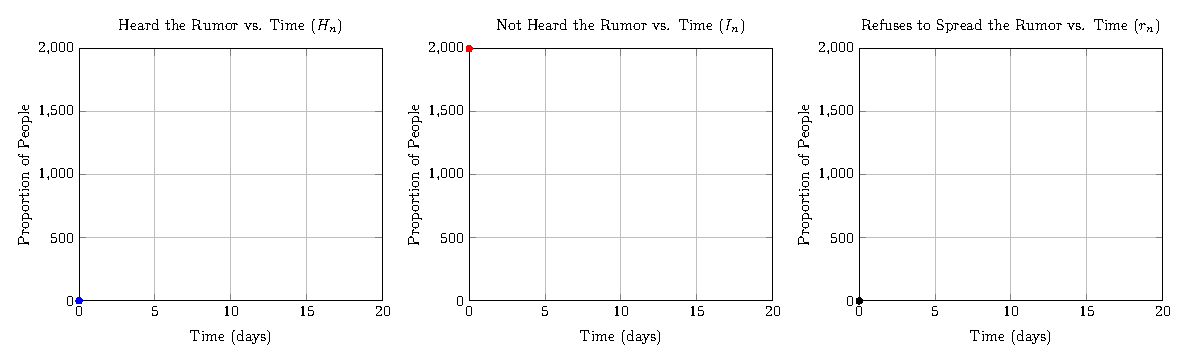
\includegraphics[width=1.0\columnwidth]{BlankAxes.eps}
    \end{center}
\end{problem}


\begin{problem}
The three sub-populations clearly trade individuals as the rumor spreads.  Since
    this is a closed system we can treat this as a {\it compartment model} where each
    state ($H$, $I$, and $R$) is connected to the other states based on how the
    transfer occurs. 

    There are several ways to organize the model.  Use Table \ref{tab:hir_table}, Table
    \ref{tab:hir_transfer}, the graphical
    representation (Figure \ref{fig:hir_graph}), and partially complete difference equations to complete the
    mathematical model. Some of the model has been completed for you to, but note that
    only one possibility is presented (feel free to change it later). The biggest
    challenge here is making conjectures about the way in which the transfers happens.

\end{problem}

        \begin{table}[ht!]
            \centering
            \begin{tabular}{|c|c|c|c|c|c|c|}
                \hline
                {\bf New Pop.} & $=$ & {\bf Old Pop.} & $+$ & {\bf Influx From} & $-$ &
                {\bf Output To} \\ \hline \hline
                Heard (new) & $=$ & Heard (old) & $+$ & Influx from Ignorant & $-$ &
                Output to Refuse \\ \hline
                Ignorant (new) & $=$ & Ignorant (old) & $+$ &  & $-$ &
                 \\ \hline
                Refuse (new) & $=$ & Refuse (old) & $+$ &   & $-$ &
                 \\ \hline
            \end{tabular}
            \caption{Table to organize transfer between compartments. Fill in the blanks.}
            \label{tab:hir_table}
        \end{table}


        \begin{table}[ht!]
            \centering
            \begin{tabular}{cc|ccc}
                & & \multicolumn{3}{|c}{{\bf From}} \\
                & & Heard & Ignorant & Refuse \\ \hline 
                \multirow{3}{*}{{\bf To}} & Heard & $-$ & proportional to $H_n \cdot I_n$
                &  \underline{\hspace{1in}} \\ 
                & Ignorant & \underline{\hspace{1in}} & $-$ & \underline{\hspace{1in}} \\
                & Refuse & proportional to $H_n$  & \underline{\hspace{1in}}  & $-$ \\ 
            \end{tabular}
            \caption{Organization table for how the populations might transfer people. Fill in the blanks.}
            \label{tab:hir_transfer}
        \end{table}


        \begin{figure}[ht!]
            \begin{center}
                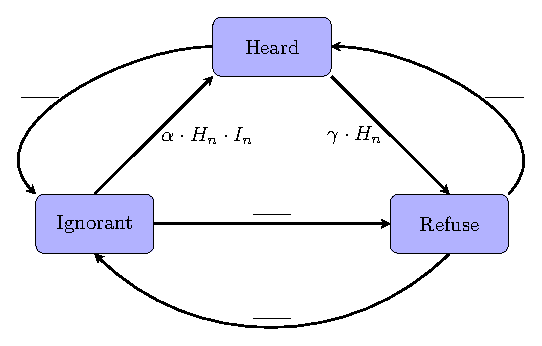
\includegraphics[width=0.5\columnwidth]{NetworkModel.eps}
            \end{center}
            \caption{A graphical representation of how the sub-populations trade people. Fill in the blanks.}
            \label{fig:hir_graph}
        \end{figure}
        
        \begin{flalign*}
            H_{n+1}-H_n &= \underline{\hspace{2in}}\\
            I_{n+1}-I_n &= \underline{\hspace{2in}}\\
            R_{n+1}-R_n &= \underline{\hspace{2in}}
        \end{flalign*}

        



        \begin{problem}
        Now we get to think about the modeling process:
            \begin{itemize}
                \item We have a mathematical model.
                \item Explicitly state your assumptions and simplifications.
                \item Determine how you might estimate each parameter in the model.
                \item Solve the mathematical model numerically using Excel (based on your
                    estimated parameters) and compare with your classmates.
                \item Analyze the results and see if they seem reasonable.
                \item Tweak the model to loosen assumptions or to more accurately model
                    reality.  This can include:
                    \begin{itemize}
                        \item allowing people to forget the rumor;
                        \item changing the way the rumor transfers;
                        \item adding more compartments; or
                        \item many other possibilities.
                    \end{itemize}
                \item Iterate this process until you think that the model approximates
                    reality.
            \end{itemize}
        \end{problem}

        \begin{problem}
            The data found
            \href{https://docs.google.com/spreadsheets/d/1jS6w4gFmxFmgaSzDaD90vDOpN2N3-DdadTxkd9pvaMI/edit?usp=sharing}{HERE} contains the proportion of the population  that has heard
            the rumor at each given time step.  Use Excel's solver along with your
            numerical model to estimate the parameters in your model.  Your end result
            should be a plot of all three population proportions.  One modeling step that
            may simplify things is that we have a closed population so we know that the
            sum of the three proportions must be 1 -- hence eliminating one of the
            populations from the model.
        \end{problem}

\newpage\section{The H1N1 Virus}
The H1N1 Virus (commonly known as Bird Flu) hit your college back in 2010.  H1N1 is a
particularly interesting virus since a infected person stays infectious for exactly 7 days
after the initial infection.  After that time the person may still be ill but is
recovering and is no longer infectious.  

\begin{problem}
    Consider a closed population of 1500 students, faculty, and staff at a small college
    campus.  On a particular day in 2010, 1 person was diagnosed with H1N1.  We'll assume
    that person was on the second day of their infectious period.  An announcement went
    out to everyone on campus to come to the health center the moment they started feeling
    symptoms.  Three days later, two new people showed up at the health center with
    symptoms.  

    Using the rather small amount of data given in the paragraph above, create a model for
    spread of the H1N1 virus through the campus.   Consider modeling the population as 9
    different compartments:
    \begin{enumerate}
        \item Susceptible,
        \item Infectious Day 1,
        \item Infectious Day 2,
        \item Infectious Day 3,
        \item Infectious Day 4,
        \item Infectious Day 5,
        \item Infectious Day 6,
        \item Infectious Day 7, and
        \item Recovered.
    \end{enumerate}
    Use Excel's Solver to find any parameters in your model.  Model first with a system of
    difference equations, then discuss with your partners whether you think it would be
    scientifically and mathematically more appropriate to use a system of differential
    equations instead.
\end{problem}


\newpage\section{Writing Systems of Difference Equations}
In order to get a great feel for setting up systems of difference equations this section
will present several examples and activities to simply get your hands dirty.  The idea
being that it takes some practice reading these problems and identifying the key
components. Each example will include some sensitivity discussion as well as a peak at the
numerical solutions. Analytical solutions are possible for some classes of systems but we
will delay this discussion until later.

\begin{example}
In the Bob Marshall Wilderness of Montana, black bears and grizzly bears compete with each
other for food.  Suppose that in the absence of any competition or hunting, the black bear
population will grow by 10\% per year, while the grizzly bear population will grow by 4\%.
Each year the competition between the two types of bears leads to the death of a certain
number of each type of bear (due to fighting and food shortages).  The number of black
bears that die is equal to the product of the black and grizzly bear populations
multiplied by $0.0003$.  The number of grizzly bears that die is equal to the product of
the black and grizzly populations multiplied by $0.0001$.  Assume that there are $1500$
black bears and $730$ grizzly bears currently present in the Bob Marshall Wilderness.
\ba
\item Write and numerically solve a pair of difference equations to model the bear populations.
\item Modify the model from part (a) to include the unfortunate fact that poachers kill
    30 black bears and 10 grizzly bears per year.
\ea
{\bf Solution:} \\
Let $B_n$ represent the population of black bears at year $n$ and $G_n$ represent the
population of grizzly bears at year $n$.  

First let us consider the black bear population.
\begin{itemize}
    \item The population of black bears increases by $10\%$ per year
    \item The population of black bears decreases from competition
\end{itemize}
With these two key features in mind the model for the black bear population is
\[ B_{n+1} = B_n + 0.10 \cdot B_n - 0.0003 B_n G_n. \]

Next let us consider the grizzly bear population.
\begin{itemize}
    \item The population of grizzly bears increases by $4\%$ per year
    \item The population of grizzly bears decreases from competition
\end{itemize}
With these two key features in mind the model for the bear population is
\[ G_{n+1} = G_n + 0.04 \cdot G_n - 0.0001 B_n G_n. \]

Obviously these two equations depend on each other because of the competition terms.
Systems that display this property are called {\it coupled}.  Putting the equations
together in one place and simplifying the algebra we see that the coupled system of
difference equations is
\begin{flalign*}
    B_{n+1} &= 1.10 \cdot B_n - 0.0003\cdot B_n\cdot G_n \\
    G_{n+1} &= 1.04 \cdot G_n - 0.0001\cdot B_n\cdot G_n
\end{flalign*}

A numerical solution of this model will result in three plots: bear population vs. time,
grizzly population vs. time, and bear population vs. grizzly population. The last of these
is called the {\it phase plot} for the system. Figure \ref{fig:9.10.ex1bears2} shows the
population dynamics for the individual bear populations.  The right-hand plot in Figure
\ref{fig:9.10.ex1bears2} shows the phase plot for the two bear populations. To read the
phase plot start at the initial condition and follow the trajectory of the points through
the phase space.  

If poaching is considered then the model becomes
\begin{flalign*}
    B_{n+1} &= 1.10 \cdot B_n - 0.0003\cdot B_n\cdot G_n - 30 \\
    G_{n+1} &= 1.04 \cdot G_n - 0.0001\cdot B_n\cdot G_n - 10
\end{flalign*}
Figure \ref{fig:9.10.ex1bears2_poach} shows the new population dynamics when poaching
occurs. 

In the non-poaching scenario it appears that the black bear population is on the rise
(over 3000 bears) and the grizzly bear population is driven to extinction.  In the
poaching scenario it appears that the black bear population reaches 600 bears after 36
years and the grizzly bears are driven to extinction within the wilderness area. Comparing
the phase plots (the right-hand figures of Figure \ref{fig:9.10.ex1bears2} and \ref{fig:9.10.ex1bears2_poach}) we
see very different dynamics with the addition of poaching.
\end{example}


\begin{figure}[ht!]
    \centering
    \begin{center}
        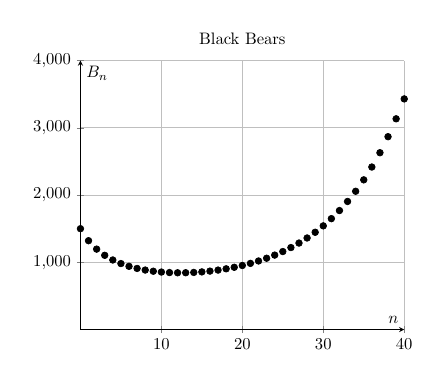
\begin{tikzpicture}[scale=0.6]
            \begin{axis}[axis lines=center, xlabel={$n$}, ylabel={$B_n$}, grid,
                title={Black Bears}, ymin=0, ymax=4000]
                \addplot[black, mark=*, only marks] coordinates{
(0 , 1500.00)
(1 , 1321.50)
(2 , 1196.08)
(3 , 1104.04)
(4 , 1034.64)
(5 , 981.46)
(6 , 940.45)
(7 , 908.90)
(8 , 884.97)
(9 , 867.36)
(10, 855.15)
(11, 847.66)
(12, 844.44)
(13, 845.16)
(14, 849.60)
(15, 857.64)
(16, 869.25)
(17, 884.46)
(18, 903.36)
(19, 926.11)
(20, 952.91)
(21, 984.06)
(22, 1019.88)
(23, 1060.80)
(24, 1107.29)
(25, 1159.94)
(26, 1219.39)
(27, 1286.40)
(28, 1361.84)
(29, 1446.71)
(30, 1542.10)
(31, 1649.28)
(32, 1769.66)
(33, 1904.79)
(34, 2056.41)
(35, 2226.41)
(36, 2416.86)
(37, 2629.98)
(38, 2868.16)
(39, 3133.95)
(40, 3430.03)};
            \end{axis}
        \end{tikzpicture}
        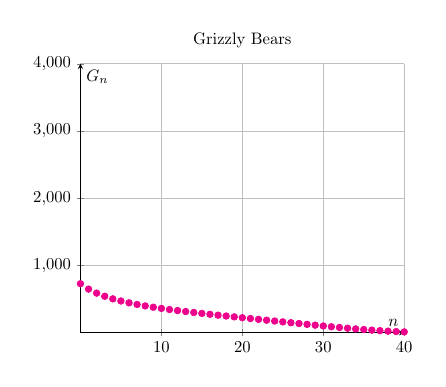
\begin{tikzpicture}[scale=0.6]
            \begin{axis}[axis lines=center, xlabel={$n$}, ylabel={$G_n$}, grid,
                title={Grizzly Bears}, ymin=0, ymax=4000]
                \addplot[magenta, mark=*, only marks] coordinates{
(0  ,730.00)
(1  ,649.70)
(2  ,589.83)
(3  ,542.88)
(4  ,504.65)
(5  ,472.63)
(6  ,445.15)
(7  ,421.09)
(8  ,399.66)
(9  ,380.28)
(10 ,362.50)
(11 ,346.00)
(12 ,330.52)
(13 ,315.83)
(14 ,301.77)
(15 ,288.20)
(16 ,275.01)
(17 ,262.11)
(18 ,249.41)
(19 ,236.85)
(20 ,224.39)
(21 ,211.98)
(22 ,199.60)
(23 ,187.23)
(24 ,174.86)
(25 ,162.49)
(26 ,150.14)
(27 ,137.84)
(28 ,125.62)
(29 ,113.54)
(30 ,101.65)
(31 ,90.04)
(32 ,78.80)
(33 ,68.00)
(34 ,57.77)
(35 ,48.20)
(36 ,39.40)
(37 ,31.45)
(38 ,24.44)
(39 ,18.41)
(40 ,13.37)};
            \end{axis}
        \end{tikzpicture}
        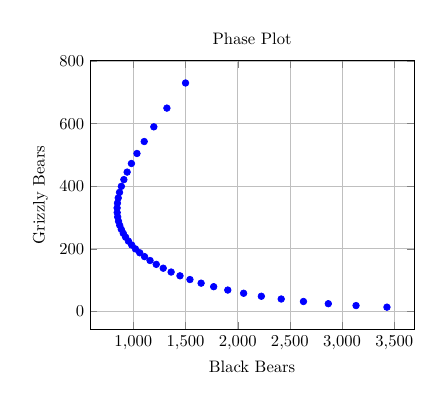
\begin{tikzpicture}[scale=0.6]
        \begin{axis}[xlabel={Black Bears}, ylabel={Grizzly Bears}, title={Phase Plot},
            grid]
            \addplot[blue, mark=*, only marks] coordinates{
(1500.00,730.00)
(1321.50,649.70)
(1196.08,589.83)
(1104.04,542.88)
(1034.64,504.65)
(981.46 ,472.63)
(940.45 ,445.15)
(908.90 ,421.09)
(884.97 ,399.66)
(867.36 ,380.28)
(855.15 ,362.50)
(847.66 ,346.00)
(844.44 ,330.52)
(845.16 ,315.83)
(849.60 ,301.77)
(857.64 ,288.20)
(869.25 ,275.01)
(884.46 ,262.11)
(903.36 ,249.41)
(926.11 ,236.85)
(952.91 ,224.39)
(984.06 ,211.98)
(1019.88,199.60)
(1060.80,187.23)
(1107.29,174.86)
(1159.94,162.49)
(1219.39,150.14)
(1286.40,137.84)
(1361.84,125.62)
(1446.71,113.54)
(1542.10,101.65)
(1649.28,90.04)
(1769.66,78.80)
(1904.79,68.00)
(2056.41,57.77)
(2226.41,48.20)
(2416.86,39.40)
(2629.98,31.45)
(2868.16,24.44)
(3133.95,18.41)
(3430.03,13.37)};
        \end{axis}
    \end{tikzpicture}
    \end{center}
    \caption{Phase plane showing the bear population dynamics}
    \label{fig:9.10.ex1bears2}
\end{figure}


\begin{figure}[ht!]
    \centering
    \begin{center}
        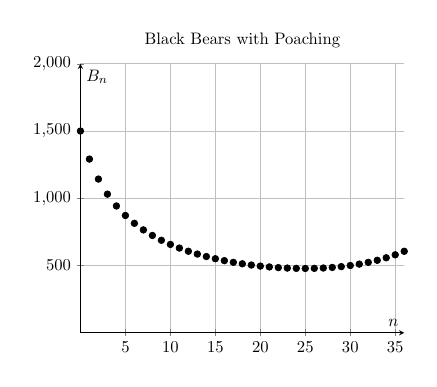
\begin{tikzpicture}[scale=0.60]
            \begin{axis}[axis lines=center, xlabel={$n$}, ylabel={$B_n$}, grid,
                title={Black Bears with Poaching}, ymin=0, ymax=2000]
                \addplot[black, mark=*, only marks] coordinates{
(0 , 1500.00)
(1 , 1291.50)
(2 , 1142.80)
(3 , 1030.74)
(4 , 942.98)
(5 , 872.25)
(6 , 813.97)
(7 , 765.11)
(8 , 723.58)
(9 , 687.88)
(10, 656.94)
(11, 629.92)
(12, 606.21)
(13, 585.34)
(14, 566.94)
(15, 550.72)
(16, 536.45)
(17, 523.96)
(18, 513.11)
(19, 503.82)
(20, 496.00)
(21, 489.61)
(22, 484.63)
(23, 481.06)
(24, 478.93)
(25, 478.27)
(26, 479.15)
(27, 481.67)
(28, 485.92)
(29, 492.04)
(30, 500.20)
(31, 510.60)
(32, 523.48)
(33, 539.09)
(34, 557.77)
(35, 579.88)
(36, 605.86)};
            \end{axis}
        \end{tikzpicture}
        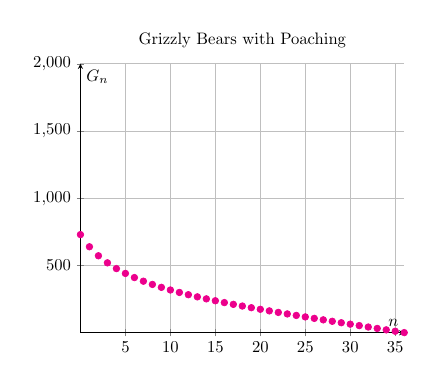
\begin{tikzpicture}[scale=0.60]
            \begin{axis}[axis lines=center, xlabel={$n$}, ylabel={$G_n$}, grid,
                title={Grizzly Bears with Poaching}, ymin=0, ymax=2000]
                \addplot[magenta, mark=*, only marks] coordinates{
(0 ,730.00)
(1 ,639.70)
(2 ,572.67)
(3 ,520.13)
(4 ,477.33)
(5 ,441.41)
(6 ,410.56)
(7 ,383.57)
(8 ,359.56)
(9 ,337.93)
(10,318.20)
(11,300.02)
(12,283.13)
(13,267.29)
(14,252.33)
(15,238.12)
(16,224.53)
(17,211.47)
(18,198.85)
(19,186.60)
(20,174.66)
(21,162.98)
(22,151.52)
(23,140.24)
(24,129.10)
(25,118.09)
(26,107.16)
(27,96.31)
(28,85.53)
(29,74.79)
(30,64.10)
(31,53.46)
(32,42.87)
(33,32.34)
(34,21.89)
(35,11.54)
(36,1.34)};
            \end{axis}
        \end{tikzpicture}
    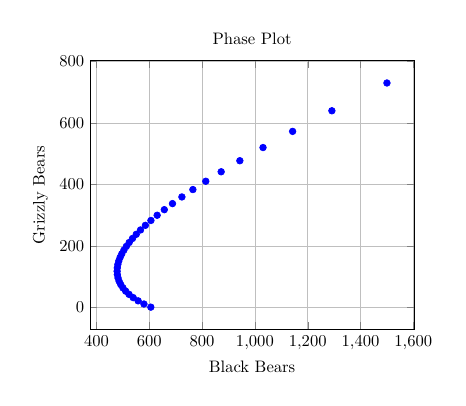
\begin{tikzpicture}[scale=0.60]
        \begin{axis}[xlabel={Black Bears}, ylabel={Grizzly Bears}, title={Phase Plot},
            grid]
            \addplot[blue, mark=*, only marks] coordinates{
(1500.00,730.00)
(1291.50,639.70)
(1142.80,572.67)
(1030.74,520.13)
(942.98 ,477.33)
(872.25 ,441.41)
(813.97 ,410.56)
(765.11 ,383.57)
(723.58 ,359.56)
(687.88 ,337.93)
(656.94 ,318.20)
(629.92 ,300.02)
(606.21 ,283.13)
(585.34 ,267.29)
(566.94 ,252.33)
(550.72 ,238.12)
(536.45 ,224.53)
(523.96 ,211.47)
(513.11 ,198.85)
(503.82 ,186.60)
(496.00 ,174.66)
(489.61 ,162.98)
(484.63 ,151.52)
(481.06 ,140.24)
(478.93 ,129.10)
(478.27 ,118.09)
(479.15 ,107.16)
(481.67 ,96.31)
(485.92 ,85.53)
(492.04 ,74.79)
(500.20 ,64.10)
(510.60 ,53.46)
(523.48 ,42.87)
(539.09 ,32.34)
(557.77 ,21.89)
(579.88 ,11.54)
(605.86 ,1.34)};
        \end{axis}
    \end{tikzpicture}
    \end{center}
    \caption{Phase plane showing the bear population dynamics}
    \label{fig:9.10.ex1bears2_poach}
\end{figure}




\begin{example}
Suppose that the past voting results of congressional elections at a certain voting
precinct are represented by the three sequences $D_n$ (Democrats), $R_n$ (Republicans),
and $T_n$ (Tea Party).  The voting behaviors of people change according to the following
observations:
\begin{center}
    \begin{tabular}{|c|c|c|}
        \hline 
        Last Year's Vote & Prediction of This Year's Vote & Percent Making This Switch \\ \hline
        \hline
        Democrat & Democrat & 70\% \\
        Democrat & Republican & 20\% \\
        Democrat & Tea Party & 10\% \\ \hline
        Republican & Republican & 50\% \\
        Republican & Democrat & 20\% \\
        Republican & Tea Party & 30\% \\ \hline
        Tea Party & Tea Party & 50\% \\
        Tea Party & Democrat & 20\% \\
        Tea Party & Republican & 30\% \\ \hline
    \end{tabular}
\end{center}
For example, the second line of the table means that $20\%$ of people that voted
democratic last time will vote republican this time. Model this scenario with a system of
difference equations.  Presume that there are 3,000 people in the precinct that are
initially split equally among the voting categories.  Is the dynamical system stable over
many years of voting supposing that the transition percentages stay the same?
\\{\bf Solution:}\\
The dynamical system needs only to keep track of how many people are in a particular
group.  Therefore the dynamical system is
\begin{flalign*}
    D_{n+1} &= 0.7 D_n + 0.2 R_n + 0.1 T_n \\
    R_{n+1} &= 0.2 D_n + 0.5 R_n + 0.3 T_n \\
    T_{n+1} &= 0.1 D_n + 0.3 R_n + 0.5 T_n
\end{flalign*}
Written in a more convenient matrix notation, this three dimensional linear system can be
written as 
\begin{flalign*}
    \begin{pmatrix} D_{n+1} \\ R_{n+1} \\ T_{n+1} \end{pmatrix} = \begin{pmatrix} 0.7 &
        0.2 & 0.1 \\ 0.2 & 0.5 & 0.3 \\ 0.1 & 0.3 & 0.5 \end{pmatrix} \cdot
        \begin{pmatrix} D_n \\ R_n \\ T_n \end{pmatrix}
\end{flalign*}
Obviously this is a three dimensional dynamical system so visualization of the numerical
solution is challenging.  There are naturally 6 two-dimensional plots that come out of the numerical
solution: $D_n$ vs $n$, $R_n$ vs $n$, $T_n$ vs $n$, $D_n$ vs $R_n$, $D_n$ vs $T_n$, and
$R_n$ vs $T_n$.  This can also be visualized in a three dimensional phase plot of $D_n$ vs
$R_n$ vs $T_n$ (we leave this to the curious reader). For simplicity we only present the
three time plots here. It is clear from Figure
\ref{fig:9.10.ex2_voting} that over the next 20 years the political parties will stabilize
at equilibrium values and the Democratic party will eventually win.  Given the obvious
volatile nature of political parties, the flawed assumption in this model is that the
transition percentages will stay fixed over the next several years.
\end{example}

\def\scl{0.6}
\begin{figure}[ht!]
    \begin{center}
        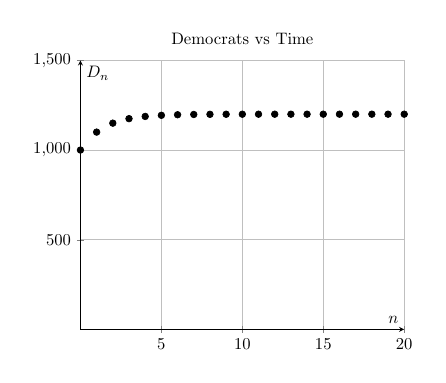
\begin{tikzpicture}[scale=0.6]
            \begin{axis}[axis lines=center, xlabel={$n$}, ylabel={$D_n$}, title={Democrats vs
                Time}, grid, ymin=0, ymax=1500]
                \addplot[black, mark=*, only marks] coordinates{(0 ,1000.00) (1 ,1100.00) (2 ,1150.00) (3 ,1175.00) (4 ,1187.50) (5 ,1193.75) (6 ,1196.87) (7 ,1198.43) (8 ,1199.21) (9 ,1199.60) (10,1199.80) (11,1199.90) (12,1199.95) (13,1199.97) (14,1199.98) (15,1199.99) (16,1199.99) (17,1199.99) (18,1199.99) (19,1200.00) (20,1200.00)};
            \end{axis}
        \end{tikzpicture}
        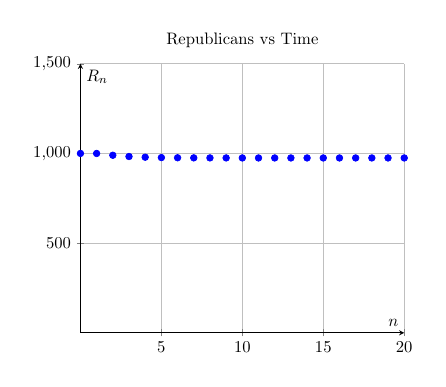
\begin{tikzpicture}[scale=0.6]
            \begin{axis}[axis lines=center, xlabel={$n$}, ylabel={$R_n$},
                title={Republicans vs Time}, grid, ymin=0, ymax=1500]
                \addplot[blue, mark=*, only marks] coordinates{(0 ,1000.000) (1 ,1000.000) (2 ,990.000) (3 ,983.000) (4 ,979.100) (5 ,977.070) (6 ,976.039) (7 ,975.520) (8 ,975.260) (9 ,975.130) (10,975.065) (11,975.033) (12,975.016) (13,975.008) (14,975.004) (15,975.002) (16,975.001) (17,975.001) (18,975.000) (19,975.000) (20,975.000)};
            \end{axis}
        \end{tikzpicture}
        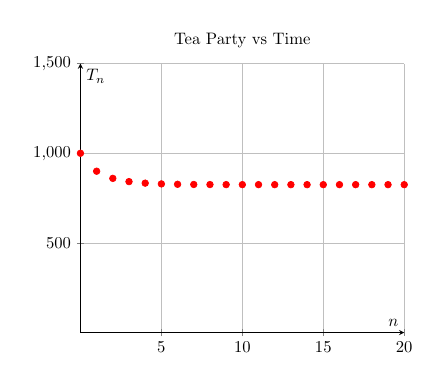
\begin{tikzpicture}[scale=0.6]
            \begin{axis}[axis lines=center, xlabel={$n$}, ylabel={$T_n$}, title={Tea Party
                vs Time}, grid, ymin=0, ymax=1500]
                \addplot[red, mark=*, only marks] coordinates{(0,1000.000) (1,900.000) (2,860.000) (3,842.000) (4,833.400) (5,829.180) (6,827.086) (7,826.042) (8,825.521) (9,825.260) (10,825.130) (11,825.065) (12,825.033) (13,825.016) (14,825.008) (15,825.004) (16,825.002) (17,825.001) (18,825.001) (19,825.000) (20,825.000)};
            \end{axis}
        \end{tikzpicture}
    \end{center}
    \caption{Numerical visualization of the voting problem. The equilibrium state appears
    to be $D_n \to 1200$, $R_n \to 975$, and $T_n \to 825$; hence giving the democrats a
clear advantage.}
    \label{fig:9.10.ex2_voting}
\end{figure}


\begin{problem}
    Bull trout and rainbow trout are prevalent fish species in Montana's rivers.  They
    have very similar feeding, migrating, and spawning habits, and as such they are in
    competition for the same food sources.  Suppose that in the absence of the other
    species in the Blackfoot River, both species would exhibit unconstrained growth.
    Since the effect of the presence of the competitor diminishes the growth rate of the
    other species, we will consider that this decrease in growth is proportional to the
    product of the size of the two competing species. Bull trout are protected in Montana
    so no fish can be legally taken from the river.  Rainbow trout, on the other hand, are
    a popular sport fish and roughly 155 rainbows are taken from the river each year by
    fishermen.  Establish a model for this interaction of the two species of fish in the
    Blackfoot River. Let $n$ be the number of years and evaluate the model over a 30 year
    span. Based on this information should fishing for bull trout be allowed?

    Use the following data for the competing trout:
    \begin{itemize}
        \item Assume equal initial populations of $2500$ fish for each species.
        \item In the absence of competition, the bull trout population increases by
            approximately 10\% per year at small populations and follow a logistic growth
            pattern otherwise with a carrying capacity of 8000 fish.
        \item In the absence of competition, the rainbow trout population increases by
            approximately 23\% per year per year at small populations and follow a
            logistic growth pattern otherwise with a carrying capacity of 8000 fish.
        \item The constant of proportionality decreasing the bull trout population is
            estimated to be approximately $0.0001$.
        \item The constant of proportionality decreasing the rainbow trout population is
            estimated to approximately $0.0001$
    \end{itemize}

\end{problem}




\begin{problem}
    In a distant country, people have only two types of breakfast cereal to eat: Corn
    Flakes and Raisin Bran. The people in this country are very loyal to their cereal and
    eat their one type of cereal every morning. Every year 200 new people join the ranks
    of Corn Flakes eaters, and 650 new people become Raisin Bran eaters every year. Of
    course sometimes people get sick of eating Corn Flakes all the time, and they switch
    to Raisin Bran. Each year about 5\% of Corn Flakes eaters switch to Raisin Bran. Write
    and solve a system of difference equations to represent the number of people eating each type of
    cereal after $n$ years. 
    \item The following system of difference equations models the populations of two types
        of animals, $A$ and $B$.
        \begin{flalign*}
            A_{n+1} &= 0.8 A_n + 0.00035 A_n B_n \\
            B_{n+1} &= 1.14 B_n - 0.00055 A_n B_n.
        \end{flalign*}
        In the absence of animal $B$ what is the rate of change of animal $A$?  In the
        absence of animal $A$ what is the rate of change of animal $B$?  How does the
        presence of animal $A$ affect the population of animal $B$?  How does the presence
        of animal $B$ affect the population of animal $A$.  How do these animals interact
        with each other?  Answer these questions first without solving the system
        numerically. Check your answers against the numerical solution.

\end{problem}



\newpage\section{Linear Systems}\label{sec:linear_systems}
The previous sections had us building models for systems of difference or differential
equations.  In this section (and for the remainder of this chapter) will will focus on a
particular type of system -- a linear system of difference or differential equations.  As
you may have guessed from the name, we will be leveraging Linear Algebra to do the
analysis on these systems.  Before we get to that let's at least build a few linear
systems.



\begin{problem}
The little town of Pudunk is filled with people who cannot make up their minds whether to
vote Democratic or Republican at the upcoming election.  Each day, 30\% of the Republicans
switch to the Democratic line, while 50\% of the Democratic voters decide to go with the
Republicans.  Assume that the population of 1000 people is initial split 50/50.
    \begin{flalign*}
        D_{n+1} - D_n = \underline{\hspace{0.5in}} D_n + \underline{\hspace{0.5in}}
        R_n\\
        R_{n+1} - R_n = \underline{\hspace{0.5in}} D_n + \underline{\hspace{0.5in}}
        R_n\\
    \end{flalign*}
\begin{itemize}
    \item[(a)] Write the system of difference equations algebraically
    \item[(b)]Write the system of difference equations using matrices
    \item[(c)] Use Excel to find a numerical solutions for the system (discuss stability if
        applicable)
\end{itemize}
\end{problem}


\begin{problem}
Deep in the redwood forest of California, dusky-footed wood rats provide up to
    80\% of the diet for the spotten owl, the main predator of the wood rat. Assume
    that initially there are 1000 rats and 10 owls.
    \begin{itemize}
        \item In the absence of wood rats, the owl population would decay by 50\% each
            year.  
        \item If rats are plentiful then the change in owl population from year
            to year will increase by 40\% of the total rat population.
        \item In the absence of owls, the population of the rats will grow by 10\% per
            year.
        \item The owls hunt the rats, so if owls are present the rate population will
            change by, let's say, 10.4\% per year.
    \end{itemize}
    \begin{flalign*}
        O_{n+1} - O_n = \underline{\hspace{0.5in}} O_n + \underline{\hspace{0.5in}}
        R_n\\
        R_{n+1} - R_n = \underline{\hspace{0.5in}} O_n + \underline{\hspace{0.5in}}
        R_n\\
    \end{flalign*}
\begin{itemize}
    \item[(a)] Write the system of difference equations algebraically
    \item[(b)]Write the system of difference equations using matrices
    \item[(c)] Use Excel to find a numerical solutions for the system (discuss stability if
        applicable)
\end{itemize}
\end{problem}


\begin{problem}
The female owls in a certain population can be classified as {\it juvenile},
    {\it subadult}, and {\it adult}. Assume that right now there are 10 juveniles, 30
    sub-adults, and 20 adults in a small owl population.  In a given year, 
    \begin{itemize}
        \item the number of new juvenile females in year $n+1$ is 0.33 times the
            number of adult females in year $n$, 
        \item 18\% of least year's juveniles becomes subadults, 
        \item 71\% of last year's subadults become adults,
        \item and 94\% of last year's adults survive.
    \end{itemize}
\begin{itemize}
    \item[(a)] Write the system of difference equations algebraically
    \item[(b)]Write the system of difference equations using matrices
    \item[(c)] Use Excel to find a numerical solutions for the system (discuss stability if
        applicable)
\end{itemize}
\end{problem}

\begin{problem}
    Two cell phone service providers, Alpha and Beta, are constantly competing for the largest market
    share. Each month 5\% of Alpha customers switch their service to Beta, and each month
    7\% of Beta customers switch their service to Alpha. The total number of customers
    served by the two companies stays fixed. 
\begin{itemize}
    \item[(a)] Write the system of difference equations algebraically
    \item[(b)]Write the system of difference equations using matrices
    \item[(c)] Use Excel to find a numerical solutions for the system (discuss stability if
        applicable)
\end{itemize}
\end{problem}

You should now have noticed that every one of the systems we've built thus far in this
section can be rewritten in the form $\bx_{n+1} = A \bx_n$.   This form is almost exactly
what we experienced from difference equations in previous chapters.  In fact, we know how
to find the solution to the difference equation $a_{n+1} = r a_n$ with initial condition
$a_0$.  Perhaps knowing how to solve the problem in one variable can give us hints about
how to solve the more general linear system.
\begin{problem}
    Work with your partner to remember how to solve the difference equation $a_{n+1} = r
    a_n$ with initial condition $a_0$. 
\end{problem}
\begin{problem}
    In modeling exercises in this section we wrote the system of difference equations as
    a matrix equation in the form: $\bx_{n+1} = A \bx_n$.  Using the same logic as
    with the previous problem, what is the analytic solution to the system of
    difference equations?
\end{problem}


Wouldn't it be nice if we had a way to {\it easily} raise a matrix to a power \dots
        
%         (and no, I'm not talking about MATLAB) \dots maybe a better question is:
%         what is matrix multiplication really doing geometrically?  Use the applet linked
%         below to play with how matrix multiplication works geometrically: \\
%         \href{https://www.geogebra.org/m/JP2XZpzV}{https://www.geogebra.org/m/JP2XZpzV}
%     \item As you play: you should notice that there are a few {\it special} vectors that
%         only get scaled by the matrix multiplication \dots keep your eyes out for these.
%         Are they always there?  How many are there?
% \end{enumerate}


\newpage\section{The Eigenvalue / Eigenvector Problem}
To answer the question posed at the end of the previous section we now turn our attention to the second fundamental question of linear algebra: $A \bx =
\lambda \bx$.  We are going to jump right in to the key definitions and we'll spend the
remainder of this section exploring these definitions.  The following two sections of the
book give details about where these ideas arise in application.

\begin{definition}
    Let $A$ be an $n \times n$ square matrix  
    \begin{itemize}
        \item An {\bf eigenvector} of the matrix $A$ is a \underline{nonzero} $n \times 1$
            vector $\bx$ such that $A\bx = \lambda \bx$.
        \item The scalar $\lambda$ is called the {\bf eigenvalue} of $A$
            associated with the eigenvector $\bx$.
    \end{itemize}
    Note that an eigenvector MUST be nonzero, but the eigenvalue MAY be zero.
\end{definition}
In simple language, If $\bx$ is an eigenvector of $A$ then $A\bx$ only scales $\bx$.  The
result of $A\bx$ will be a vector parallel to $\bx$, so no rotations (other than
180$^\circ$) result.

% \input{previews/10.6.PA1}
\begin{problem}
    Consider the matrix $A= \bpm -7 & 9 \\ -6 & 8 \epm$.
\ba
    \item Is $\bx = \bpm 1 \\ 1 \epm$ an eigenvector for $A$?  If so, what is the
        associated eigenvalue?  If not, why not?
    \item Is $\bu = \bpm 3 \\ -2 \epm$ an eigenvector for $A$?  If so, what is the
        associated eigenvalue?  If not, why not?
    \item Is $\bv = \bpm 3 \\ 2 \epm$ an eigenvector for $A$?  If so, what is the
        associated eigenvalue?  If not, why not?
    \item Is $\by = \bpm -1 \\ 1 \epm$ an eigenvector for $A$?  If so, what is the
        associated eigenvalue?  If not, why not?
    \item The plot below shows the four vectors considered in parts (a) - (d) of this
        problem.  Sketch $A\bx$, $A\bu$, $A\bv$, and $A\by$ on the same coordinate
        plane, indicate which vectors are eigenvectors, and indicate the eigenvalues
        geometrically.
        \begin{center}
            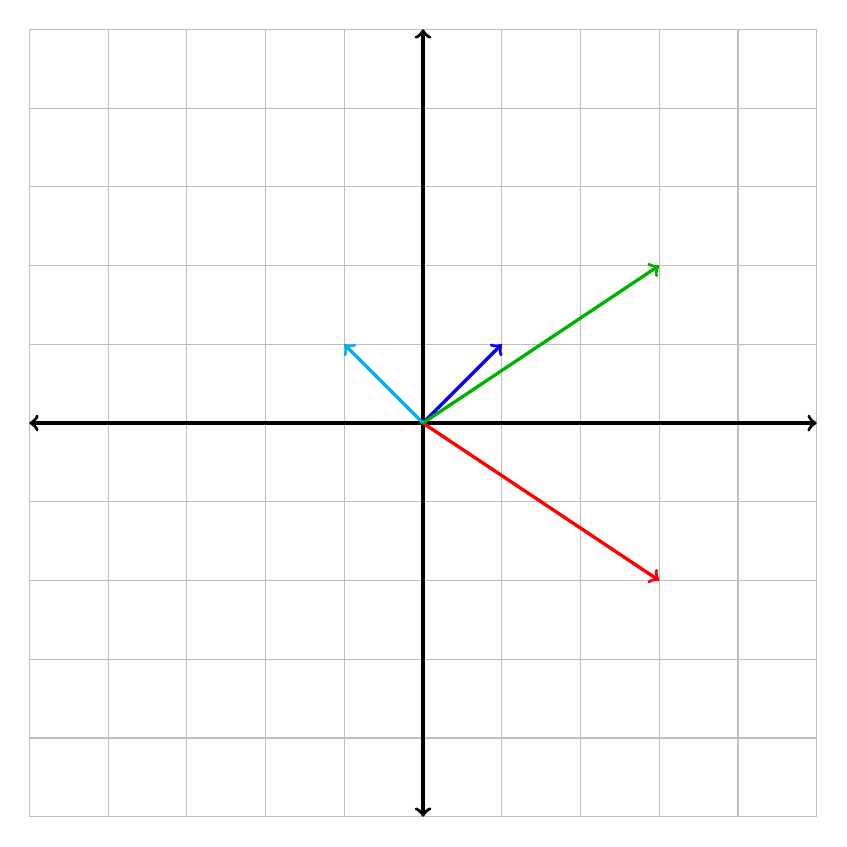
\begin{tikzpicture}
                \draw[color=gray!50] (-5,-5) grid (5,5);
                \draw[very thick, black, <->] (-5,0) -- (5,0);
                \draw[very thick, black, <->] (0,-5) -- (0,5);
                \draw[very thick, blue, ->] (0,0) -- (1,1) node[anchor=south]{$\bx$};
                \draw[very thick, red, ->] (0,0) -- (3,-2) node[anchor=west]{$\bu$};
                \draw[very thick, green!70!black, ->] (0,0) -- (3,2) node[anchor=west]{$\bv$};
                \draw[very thick, cyan, ->] (0,0) -- (-1,1) node[anchor=east]{$\by$};
            \end{tikzpicture}
        \end{center}
\ea
\end{problem}

% \input{activities/10.6.Act1}
\begin{problem}
    Use the GeoGebra applet
    \href{http://www.geogebratube.org/student/m334841}{http://www.geogebratube.org/student/m334841}
    to explore the following questions.
    \ba
        \item Approximate the eigenvalue-eigenvector pairs for the matrix $\bpm 0 & 2 \\ 1
            & -1 \epm$.
        \item Approximate the eigenvalue-eigenvector pairs for the matrix $\bpm 1 & 2 \\ 0
            & -3 \epm$.
        \item Approximate the eigenvalue-eigenvector pairs for the matrix $\bpm 0.25 & 0.1
            \\ 0.75 & 0.9 \epm$.
    \ea

\end{problem}

\subsection{Geometry of Eigenvectors and Eigenvalues}
In the introduction to this section we saw that an eigenvector of a matrix is only scaled
by the matrix.  This simple geometric fact leads us to the fact that if you know all of
the eigenvalue / eigenvector information about a matrix, you can determine its full
behavior on any vector.  This leads us to the following theorem.

\begin{thm}\label{thm:10.6.eig1}
    Let $A$ be an $n \times n$ matrix with eigenvectors $\bv_1, \bv_2, \dots, \bv_n$ and
    associated eigenvalues $\lambda_1, \lambda_2, \dots, \lambda_n$.  If $\bu$ is an
    $n$-dimensional vector and we can write $\bu$ as a linear combination of the
    eigenvectors 
    \[ \bu = c_1 \bv_1 + c_2 \bv_2 + \cdots c_n \bv_n, \]
    then we know the action of $A$ on $\bu$
    \[ A\bu = A\left(c_1 \bv_1 + c_2 \bv_2 + \cdots c_n \bv_n\right) = c_1 \lambda_1 \bv_1
        + c_2 \lambda_2 \bv_2 + \cdots c_n \lambda_n \bv_n. \]
\end{thm}

The following example illustrates this idea.
\begin{example}
Let $\bv_1 = \bpm 0 \\ -3 \\ 1 \epm$, $\bv_2 = \bpm 1 \\ 3 \\ 0 \epm$, and $\bv_3 = \bpm 2
\\ 0 \\ -1 \epm$ be eigenvectors of the matrix $A$ with corresponding eigenvalues
$\lambda_1 = -2$, $\lambda_2 = -1$, and $\lambda_3 = 0$.  
If $\bu = \bpm 3 \\ -3 \\ 1 \epm$ then what is $A\bu$?
\\{\bf Solution:} \\
Since we know all of the information about the eigenvectors, if we can write $\bu$ as a
linear combination of the eigenvectors then we can easily determine $A\bu$.  

We need to find $c_1, c_2,$ and $c_3$ such that $\bu = c_1 \bv_1 + c_2 \bv_2 + c_3 \bv_3$.
This is a system of equation, and we can write the matrix form of this system as
\[ \bpm 0 & 1 & 2 \\ -3 & 3 & 0 \\ 1 & 0 & -1 \epm \bpm c_1 \\ c_2 \\ c_3 \epm = \bpm 3 \\
    -3 \\ 1 \epm. \]
Augmenting this system and row reducing gives
\[ \left( \begin{array}{ccc|c} 0 & 1 & 2 & 3 \\ -3 & 3 & 0 & -3 \\ 1 & 0 & -1 & 1
    \end{array} \right) \to \cdots \to \left( \begin{array}{ccc|c} 1 & 0 & 0 & 2 \\ 0 & 1
        & 0 & 1 \\ 0 & 0 & 1 & 1 \end{array} \right) \]
Therefore, 
\[ \bu = 2 \bv_1 + 1\bv_2 + 1 \bv_3 \]
and 
\[ A\bu = 2 \lambda_1 \bv_1 + 1 \lambda_2 \bv_2 + 1 \lambda_3 \bv_3 = -4 \bv_1 - \bv_2 =
    \bpm -1 \\ 9 \\ -4 \epm \]
Notice that this was done with NO knowledge of $A$ itself.
\end{example}


In the previous example it wasn't necessary to find the matrix $A$.  In some applications
the eigenvalues and eigenvectors are well known but the matrix is actually needed.  The
following example illustrates how to work backwards from eigen-information to the matrix.

\begin{example}
Assume that $\bv_1 =\bpm 2 \\ -3 \epm$ and $\bv_2 = \bpm 1 \\ -1 \epm$ are the
eigenvectors of a matrix $A$ with eigenvalues $\lambda_1 = 3$ and $\lambda_2 = -2$.  What
is the matrix $A$?
\\{\bf Solution:}\\
We know that $A$ is a $2 \times 2$ matrix so we can write $A = \bpm a & b \\ c & d \epm$.
We know that $A \bv_1 = \lambda_1 \bv_1$ and $A \bv_2 = \lambda_2 \bv_2$, and out of these
equations we can write a system of four equations with unknowns $a,b,c$, and $d$.
\begin{align*}
    A\bv_1 = \lambda_1 \bv_1 &\quad \implies \quad \left\{\begin{array}{rl} 2a-3b &= 6 \\ 2c-3d
        &= -9 \end{array} \right. \\
    A\bv_2 = \lambda_2 \bv_2 &\quad \implies \quad \left\{ \begin{array}{rl} 1a-1b &= -2 \\ 1c-1d
        &= 2 \end{array} \right.
\end{align*}
The augmented $4 \times 4$ system of equations is
\[ \left( \begin{array}{cccc|c} 2 & -3 & 0 & 0 & 6 \\
                                0 & 0 & 2 & -3 & -9 \\
                                1 & -1 & 0 & 0 & -2 \\
                                0 & 0 & 1 & -1 & 2 \end{array} \right) 
    \to \cdots \to
    \left( \begin{array}{cccc|c} 1 & 0 & 0 & 0 & -12 \\
                                 0 & 1 & 0 & 0 & -10 \\
                                 0 & 0 & 1 & 0 & 15 \\
                                 0 & 0 & 0 & 1 & 13 \end{array} \right)
        \]
Therefore, 
\[A = \bpm -12 & -10 \\ 15 & 13 \epm \]
\end{example}

Another advantage to eigenvalue / eigenvector information is the ability to easily examine
powers of a matrix.  This will be especially important when examining time-dependent
matrix systems where the exponent represents steps in time.
\begin{thm}\label{thm:10.6.ev2}
    If $A$ is an $n \times n$ matrix, $\lambda$ is an eigenvalue of $A$ and $\bv$ is the
    associated eigenvector, then 
    \[ A^k \bv = \lambda^k \bv \]

    Furthermore,
    If $A$ has eigenvalues $\lambda_1, \lambda_2, \ldots, \lambda_n$ and eigenvectors
    $\bv_1, \bv_2, \ldots, \bv_n$ then if $\bu$ is an $n$-dimensional vector with $\bu =
    c_1 \bv_1 + c_2 \bv_2 + \cdots c_n \bv_n$, then
    \[ A^k \bu = c_1 \lambda_1^k \bv_1 +c_2 \lambda_2^k \bv_2 + \cdots c_n \lambda_n^k
        \bv_n. \]
    
\end{thm}

\begin{example}
Let $A$ have eigenvalues $\lambda_1 = 4$ and $\lambda_2 = 0.1$ with eigenvectors $\bv_1 =
\bpm 1 \\ -2 \epm$ and $\bv_2 = \bpm 3 \\ 5 \epm$.  Explore the quantities $A^k \bv_1$ and
$A^k \bv_2$ for various values of $k$.
\\{\bf Solution:}\\
From Theorem \ref{thm:10.6.ev2} we know that $A^k \bv_j = \lambda_j^k \bv_j$.  Therefore
\[ A^k \bv_1 = 4^k \bpm 1 \\ -2 \epm = \bpm 4^k \\ -2 \cdot 4^k \epm. \]
Similarly,
\[ A^k \bv_2 = (0.1)^k \bpm 3 \\ 5 \epm = \bpm 3 \cdot (0.1)^k \\ 5 \cdot (0.1)^k \epm. \]
For larger and larger values of $k$, the entries of $A^k \bv_1$ grow exponentially and the
values of $A^k \bv_2$ decay exponentially to zero.
\end{example}

% \input{activities/10.6.Act2}
\begin{problem}
    Use the geometry and definitions of eigenvectors and eigenvalues to answer the
    following questions.
    \ba
        \item Given that $\bv_1 = \bpm 1 \\ -2 \epm$ and $\bv_2 = \bpm -1 \\ 1 \epm$ are
            the eigenvectors of the matrix $A = \bpm -2 & 1 \\ -2 & -5 \epm$, what are the
            corresponding eigenvalues?
        \item Find the $2 \times 2$ matrix $A$ such that $\bv_1 = \bpm -1 \\ 1 \epm$ and
            $\bv_2 = \bpm -4 \\ 1 \epm$ are the eigenvectors of $A$ with eigenvalues $6$
            and $3$ respectively.
        \item If $\bv_1 = \bpm 2 \\ -3 \epm$ and $\bv_2 = \bpm 5 \\ 1 \epm$ are the
            eigenvectors of a matrix $A$ with corresponding eigenvalues $\lambda_1 = 2$
            and $\lambda_2 = 5$, then what is $A(2\bv_1 + 5\bv_2)$?
        \item Let $\bv_1 = \bpm 2 \\ -3 \epm$ and $\bv_2 = \bpm 5 \\ 1 \epm$ be the
            eigenvectors of a matrix $A$ with corresponding eigenvalues $\lambda_1 = 2$
            and $\lambda_2 = 5$.  If $\bu = \bpm 17 \\ 0 \epm$, what is $A\bu$? Hint:
            Find $c_1$ and $c_2$ such that $\bu = c_1 \bv_1 + c_2 \bv_2$.
        \item If $\bv_1 = \bpm 6 \\ 4 \epm$ and $\bv_2 = \bpm 1 \\ -3 \epm$ are the
            eigenvectors of $A$ with eigenvalues $\lambda_1 = 3$ and $\lambda_2 =
            \frac{1}{2}$,
            find $A^5 \bv_1$ and $A^5 \bv_2$.
        \item If $\bv_1 = \bpm 6 \\ 4 \epm$ and $\bv_2 = \bpm 1 \\ -3 \epm$ are the
            eigenvectors of $A$ with eigenvalues $\lambda_1 = 3$ and $\lambda_2 =
            \frac{1}{2}$,
            find $\lim_{k \to \infty} \left( A^k \bv_1 \right)$ and $\lim_{k\to \infty}
            \left( A^k \bv_2 \right)$.
    \ea

\end{problem}


\subsection{The Eigenvalue Eigenvector Problem}
Given a matrix and a vector it is easy to determine if the vector is an eigenvector.  If,
on the other hand, we try to extract the eigenvectors and eigenvalues from a given matrix
the problem is a bit more interesting.  We want to solve $A\bx = \lambda \bx$ for $\bx$,
but the unknown is on both sides of the equation.  Doing a bit of (linear) algebra we can
rearrange the equation to get
\begin{flalign}
    A \bx = \lambda \bx \quad \implies \quad A \bx - \lambda \bx = 0 \quad
    \implies \quad \left( A - \lambda I \right) \bx = 0.
    \label{eqn:10.6.evev1}
\end{flalign}
The last equation of \eqref{eqn:10.6.evev1} says something very profound about the matrix
$A - \lambda I$ when $\lambda$ is an eigenvalue: this matrix must NOT have an inverse!
From our properties of determinants, this means that we must have
\[ \det\left( A - \lambda I \right) = 0. \]
This determinant will be an $n^{th}$-order polynomial equation in $\lambda$.
\begin{definition}
    The {\bf characteristic polynomial} of a square matrix $A$ is given by
    \[ p(\lambda) = \det\left( A - \lambda I \right). \]
    If $A$ is $n \times n$ then 
    \[ p(\lambda) = c_n \lambda^n + c_{n-1} \lambda^{n-1} + \cdots + p_1 \lambda + p_0. \]
\end{definition}
We now have a way to find the eigenvalues of a matrix. The process is outlined in
Theorem \ref{thm:eigen_process}.

\begin{thm}
    Let $A$ be an $n \times n$ matrix.  To find the eigenvalues and eigenvectors of $A$
    \begin{enumerate}
        \item Find the characteristic polynomial $p(\lambda) = \det(A-\lambda I)$.
        \item Set the characteristic polynomial to zero to get the characteristic equation
            \[ \det(A - \lambda I)=0. \]
        \item Solve the characteristic equation for all values of $\lambda$. These are the
            eigenvalues of $A$.
        \item For each eigenvalue $\lambda$, find $\bx$ such that $(A-\lambda I) \bx =
            0$.  The nonzero solution to this system of equations is the
            eigenvector of $A$ associated with the eigenvalue $\lambda$.
    \end{enumerate}
    \label{thm:eigen_process}
\end{thm}

The observant reader should note that step 3 of the eigenvalue process is often very
difficult or simply impossible to do by hand.  This is the step that makes the eigenvalue
/ eigenvector problem so difficult! For a $2 \times 2$ matrix, the characteristic equation
is quadratic and there is a convenient formula to find the roots.  For a $3 \times 3$
matrix the characteristic polynomial is cubic.  There is a formula to solve the general
cubic similar to the quadratic formula (due to Gerolamo Cardano in the early 1500's), but
it is quite cumbersome to use.  For a $4 \times 4$ matrix the characteristic polynomial is
quartic.  Like the previous two cases, there is a general formula (due to Lodovico Ferrari
in the 1500's) that solves the general quartic.  At this point, the reader may think that
there are general formulas to solve most polynomial equations.  Unfortunately, that is
simply false!  In the 1800's, \'Evariste Galois showed that there can not be any such
formula for the general quintic polynomial!\footnote{Galois' discovery paved the way for
an entire field of study called Abstract Algebra.}  This amazing fact has a huge impact on the
search for eigenvalues: If you are dealing with a $5\times 5$ matrix there is not way to
get a general solution to the resulting characteristic equation, and a $5 \times 5$ matrix
is very small!!

The preceding paragraph leads us to two conclusions:
\begin{enumerate}
    \item To find the eigenvalues of a matrix by hand we need to be dealing with small
        matrices.
    \item To find the eigenvalues of a larger matrix, we need computational methods that
        will allow us to approximate the roots of polynomials.  
\end{enumerate}
For now, we'll stick with small examples just to get the hang of the algorithm.  Let's
examine a few examples of the eigenvector / eigenvalue problem.  Work along with these
examples so that you understand every step.

\begin{example}
Find the eigenvalue eigenvector pairs for the matrix $A = \bpm 2 & 7 \\ 7 & 2 \epm$.
\\{\bf Solution:}\\
The characteristic polynomial of $A$ is 
\[ p(\lambda) = \det \left( \bpm 2 & 7 \\ 7 & 2 \epm - \lambda \bpm 1 & 0 \\ 0 & 1 \epm
    \right) = \det \left( \bpm 2-\lambda & 7 \\ 7 & 2-\lambda \epm \right) = \left( 2-\lambda
    \right)^2 - 49 \]
If we now set the characteristic polynomial to zero and solve we get
\begin{flalign*}
    & p(\lambda) =0 \\
    &\implies (2-\lambda)^2-49=0 \\
    &\implies (2-\lambda)^2=49 \\
    &\implies 2-\lambda=\pm 7 \\
    &\implies -\lambda=-2 \pm 7 \\
    &\implies \lambda=2 \pm 7 \\
    & \implies \lambda_1 = 9 \quad \text{and} \quad \lambda_2 = -5.
\end{flalign*}

Now we need to find the two associated eigenvectors.  
\begin{description}
    \item[For $\lambda_1=9$:] We need to solve $(A-\lambda_1 I) \bx= 0$.
        First, $A-\lambda_1 I = \bpm -7 & 7 \\ -7 & 7 \epm$, so augmenting this with the
        zero vector and row reducing gives
        \[ (A-\lambda_1 I \, | \, 0) = \left( \begin{array}{cc|c} -7 & 7 & 0 \\ 7 & -7 & 0
            \end{array} \right) \to \left( \begin{array}{cc|c} 1 & -1 & 0 \\ 0 & 0 & 0
            \end{array} \right). \]
        Therefore if $\bx = \bpm x_1 \\ x_2 \epm$ then $x_1 = x_2$ and the simplest
        nonzero vector describing this is $\bx = \bpm 1 \\ 1 \epm$.  The reader should
        verify that $A\bpm 1 \\ 1 \epm = 9 \bpm 1 \\ 1 \epm$ 

    \item[For $\lambda_2=-5$:] We need to solve $(A - \lambda_2 I) \bx = 0$.
        First, $A - \lambda_2 I = \bpm 7 & 7 \\ 7 & 7 \epm$, so augmenting this with the
        zero vector and row reducing gives
        zero vector and row reducing gives
        \[ (A-\lambda_2 I \, | \, 0) = \left( \begin{array}{cc|c} 7 & 7 & 0 \\ 7 & 7 & 0
            \end{array} \right) \to \left( \begin{array}{cc|c} 1 & 1 & 0 \\ 0 & 0 & 0
            \end{array} \right). \]
        Therefore if $\bx = \bpm x_1 \\ x_2 \epm$ then $x_1 = -x_2$ and the simplest
        nonzero vector describing this is $\bx = \bpm 1 \\ -1 \epm$.  The reader should
        verify that $A\bpm 1 \\ -1 \epm = (-5) \bpm 1 \\ -1 \epm$ 
\end{description}
The eigenvalue / eigenvector pairs for $\bpm 2 & 7 \\ 7 & 2 \epm$ are
\[ \lambda_1 = 9 \text{ with } \bx_1 = \bpm 1 \\ 1 \epm \quad \text{and} \quad \lambda_2 =
    -5 \text{ with } \bx_2 = \bpm 1 \\ -1 \epm. \]
\end{example}

In the next example we illustrate a convenient shortcut when the matrix has triangular
structure.
\begin{example}
For $A = \bpm 5 & 5 & 0 & 5 \\0 & 2 & -3 & 6 \\ 0 & 0 & 3 & -2 \\0 & 0 & 0 & 5 \epm$, find
the eigenvalues and eigenvectors.
\\{\bf Solution:}\\
Notice that the matrix $A$ is upper triangular.  This means that $A-\lambda I$ is upper
triangular and the determinant is the product of the diagonal entries.  Hence, the
characteristic polynomial is
\[ p(\lambda) = (5-\lambda)(2-\lambda)(3-\lambda)(5-\lambda). \]
The resulting characteristic equation $p(\lambda)=0$ is very easy to solve giving
$\lambda_1 = 5$, $\lambda_2 = 2$, and $\lambda_3=3$.
\begin{description}
    \item[For $\lambda_1=5$:] We form the homogeneous system $(A-5I)\bx = 0$,
        augment, and row reduce to get
        \[ \left( \begin{array}{cccc|c} 0 & 5 & 0 & 5 & 0 \\
                                        0 & -3 & -3 & 6& 0 \\
                                        0 & 0 & -2 & -2 & 0 \\
                                        0 & 0 & 0 & 0 & 0 \end{array} \right) 
%         \to
%         \left( \begin{array}{cccc|c} 0 & 1 & 0 & 1 & 0 \\
%                                         0 & 1 & 1 & -2& 0 \\
%                                         0 & 0 & 1 & 1 & 0 \\
%                                         0 & 0 & 0 & 0 & 0 \end{array} \right)
%         \to
%         \left( \begin{array}{cccc|c} 0 & 1 & 0 & 1 & 0 \\
%                                         0 & 1 & 0 & -3& 0 \\
%                                         0 & 0 & 1 & 1 & 0 \\
%                                         0 & 0 & 0 & 0 & 0 \end{array} \right)
        \to \cdots \to
        \left( \begin{array}{cccc|c} 0 & 1 & 0 & 0 & 0 \\
                                     0 & 0 & 1 & 0& 0 \\
                                        0 & 0 & 0 & 1 & 0 \\
                                        0 & 0 & 0 & 0 & 0 \end{array} \right)
        \]
        Hence, if $\bx = \bpm x_1 \\ x_2 \\ x_3 \\ x_4 \epm$ then $x_2=x_3=x_4=0$ and
        $x_1$ is free.  Taking $x_1=1$ we get $\bx = \bpm 1 \\ 0 \\ 0 \\
        0 \epm$.  The reader should verify that $\lambda_1 = 5$ and $\bx = (1,0,0,0)^T$ is indeed an eigenvalue /eigenvector
        pair for the matrix $A$.
    \item[For $\lambda_2=2$:] We form the homogeneous system $(A-2I)\bx=0$,
        augment, and row reduce to get
        \[ \left( \begin{array}{cccc|c} 3 & 5 & 0 & 5 & 0 \\
                                        0 & 0 & -3 & 6& 0 \\
                                        0 & 0 & 1 & -2 & 0 \\
                                        0 & 0 & 0 & 3 & 0 \end{array} \right) 
        \to \cdots \to
        \left( \begin{array}{cccc|c} 1 & \frac{5}{3} & 0 & 0 & 0 \\
                                    0 & 0 & 1 & 0 & 0 \\
                                    0 & 0 & 0 & 1 & 0 \\
                                    0 & 0 & 0 & 0 & 0 \end{array} \right).
        \]
        Therefore, $x_3=x_4=0$, $x_2$ is free, and $x_1 = -\frac{5}{3} x_2$.  Picking
        $x_4=3$ (for convenience) we see that $\bx = \bpm -5 \\3\\0\\0\epm$ is the
        eigenvector associated with $\lambda_2=2$.
    \item[For $\lambda_3=3$:] We form the homogeneous system $(A-3I)\bx = 0$,
        augment, and row reduce to get
        \[ \left( \begin{array}{cccc|c} 2 & 5 & 0 & 5 & 0 \\
                                        0 & -1 & -3 & 6& 0 \\
                                        0 & 0 & 0 & -2 & 0 \\
                                        0 & 0 & 0 & 2 & 0 \end{array} \right) 
        \to \cdots \to
        \left( \begin{array}{cccc|c} 1 & 0 & -\frac{15}{2} & 0 & 0 \\
                                    0 & 1 & 3 & 0 & 0 \\
                                    0 & 0 & 0 & 1 & 0 \\
                                    0 & 0 & 0 & 0 & 0 \end{array} \right).
        \]
        Hence, $x_4=0$, $x_3$ is free, $x_2=-3x_3$, and $x_1 = \frac{15}{2} x_3$.  Picking
        $x_3=2$ (for convenience) gives $\bx = \bpm 15 \\ -6 \\ 2 \\ 0 \epm$.
\end{description}
Therefore, the eigenvalue / eigenvector pairs are
\[ \lambda_1 = 5 \text{ with } \bx_1 = \bpm 1 \\ 0 \\ 0 \\ 0 \epm, \quad \lambda_2=2
    \text{ with } \bx_2 = \bpm -5 \\ 3 \\ 0 \\ 0 \epm, \quad \text{and} \quad \lambda_3 =
    3 \text{ with } \bx_3 = \bpm 15 \\ -6 \\ 2 \\ 0 \epm \]
Notice that in this problem the matrix was $4 \times 4$ but there are only three
eigenvalue / eigenvector pairs.  This occasionally occurs with repeated roots in the
characteristic polynomial.  
\end{example}
 
% \input{activities/10.6.Act3}
\begin{problem}
    Find the eigenvectors and eigenvalues for each of the following matrices.
    \ba
        \item $A = \bpm -4 & -1 \\ 6 & 1 \epm$
        \item $B = \bpm 5 & 3 \\ 2 & 0 \epm$
        \item $C = \bpm 3 & 0 & 0 \\ 6 & 2 & 0 \\ 0 & 3 & 6 \epm$
        \item $D = \bpm 4 & 0 & -1 \\ 0 & 4 & -1 \\ 1 & 0 & 2 \epm$
    \ea

\end{problem}




 



\subsection{Technology for the Eigenvalue Eigenvector Problem}
Linear algebra software is designed to handle the eigenvalue-eigenvector problem with
refined efficiency.  Based on the length of the computations in this section it is clear
that some technological aid is necessary for many eigvalue-eigenvector computations.  In
this final subsection we will illustrate how MatLab computes eigenvalues and eigenvectors.

\begin{example}
Consider the matrix 
\[ A = \bpm 26  & -18 & 6 \\ 18.5 & -11 & 5.5 \\ -26 & 22 & -2 \epm. \]
Use MatLab to find the eigenvalues and eigenvectors.
\\{\bf Solution:}\\
The MatLab code is shown below.  The function \texttt{eig} is the command that finds the
eigen-pairs.
\begin{verbatim}
A = 26 , -18 , 6 ; 
    18.5 , -11 , 5.5 ;
    -26 , 22 , -2];
[vectors , values] = eig(A)
\end{verbatim}

The output to the MatLab command line is:
\begin{verbatim}
vectors =
 0.5774    0.3906    0.4851
 0.5774    0.1302    0.7276
-0.5774   -0.9113    0.4851

values =
2.0000         0         0
0              6.0000    0
0              0         5.0000
\end{verbatim}

The eigenvalue and eigenvector pairs in the matrix are
\[ \lambda_1 = 2 \text{ with } \bv_1 = \bpm 1 \\ 1 \\ -1 \epm, \quad \lambda_2 = 6
    \text{ with } \bv_2 = \bpm 3 \\ 1 \\ -7 \epm, \quad \text{ and } \lambda_3=5 \text{
    with } \bv_3 = \bpm 2 \\ 3 \\ 2\epm. \]
Reading the values from the eigenvectors is a bit tricky.  MatLab scales the vectors so
that the magnitude is 1 so to get integer values out of the eigenvectors (if that is
possible) it is a matter of looking at the relative weights of the values.  For example,
in $\bv_1$, the numbers are all the same so they might as well be $1$.  In $\bv_2$, on the
other hand, taking the smallest value to be 1 we see that the middle value is three times
as large and the negative values is seven times as large.
\end{example}

\newpage\section{Markov Chains}
\begin{problem}\label{prob:bull_bear}
    The stock market can be divided into three behaviors:

    \begin{minipage}{0.4\columnwidth}
    \begin{itemize}
        \item A bull market is a period of generally rising prices.
        \item A bear market is a period of generally declining prices.
        \item A stagnant market is a period of generally no rise or decline of prices.
    \end{itemize}
    The graph at right shows how the markets evolve over time. For example, a bull week is
    followed by a bull week 90\% of the time, a bear week 7.5\% of the time, and a
    stagnant week 2.5\% of the time.
\end{minipage}
\begin{minipage}{0.55\columnwidth}
    \begin{center}
       \begin{tikzpicture}[->,>=stealth',shorten >=1pt,auto,node distance=4cm,
  thick,main node/.style={circle,fill=blue!20,draw,font=\sffamily}]
        \node[main node] (bear) {Bear};
        \node[main node] (bull) [below right of=bear] {Bull};
        \node[main node] (stag) [below left of=bear] {Stag};
        \path[every node/.style={font=\sffamily\small}]
            (bear) edge [loop above] node {0.8} (bear)
                   edge [bend right] node[right] {0.15} (bull)
                   edge [bend left] node[left] {0.05} (stag)
            (bull) edge [loop right] node {0.9} (bull)
                   edge [bend right] node[right] {0.075} (bear)
                   edge [bend left] node[below] {0.025} (stag)
            (stag) edge [loop left] node {0.5} (stag)
                   edge [bend left] node[left] {0.25} (bear)
                   edge node[above] {0.25} (bull);
\end{tikzpicture} 
    \end{center}
\end{minipage}

    \ba
        \item Fill in the table below to create a {\it transition matrix} indicating how
            the market transitions over time.
            \begin{center}
                \begin{tabular}{l|ccc}
                    & From Bull & From Bear & From Stagnant \\ \hline 
                    To Bull & & & \\
                    To Bear & & & \\
                    To Stagnant & & & 
                \end{tabular}
            \end{center}

        \item Verify that the sum of every column is exactly 1.  Why is this important?
        \item If we know that we are in a bull market this week, what is the probability
            of being in each type of market next week? What if this week were a bear
            market?  What about a stagnant market? \\ Hint: This can be calculated by
            simple matrix multiplication.
        \item If we are in a bull market right now, what is the probability that we'll be
            in a bull market 10 weeks from now?
    \ea

\end{problem}
% \input{previews/10.7.PA1}


% \subsection*{Markov Chains}
In Problem \ref{prob:bull_bear} we saw our first example of a stochastic matrix and a
Markov chain.  The formal definitions are as follows.
\begin{definition}\label{def:10.7.markov}
    \begin{itemize}
        \item A {\bf probability vector} is a vector with nonnegative entries that add to
            1.
        \item A {\bf stochastic matrix} is a matrix whose columns are probability vectors.
        \item A {\bf Markov chain} is a sequence of probability vectors $\bx_0, \bx_1,
            \bx_2, \dots$ together with a stochastic matrix $P$ such that
            \[ \bx_1 = P\bx_0, \quad \bx_2 = P\bx_1, \quad \bx_3 = P \bx_2, \quad \ldots.
                \]
            Note that a Markov chain is most simply written as the first order linear
            difference equation 
            \[ \bx_{k+1} = P \bx_k \quad \text{ for } k=0, 1, 2, \dots. \]
    \end{itemize}
\end{definition}

A Markov chain is a tool used in many fields to understand long-term probability in a
closed system.  In Definition \ref{def:10.7.markov} we see that the Markov chain of
probabilities can be stated as a discrete dynamical system $\bx_{k+1} = P \bx_k$.  Hence
we can determine the probability of being in any state at a given time by observing Table
\ref{tab:10.7.markov}.
\begin{table}[ht!]
    \begin{center}
        \begin{tabular}{|c|c|c|}
            \hline
            $k$ & $\bx_{k+1}$ & $P\bx_k$ \\ \hline \hline
            0 & $\bx_1$ & $P\bx_0$ \\
            1 & $\bx_2$ & $P\bx_1 = P(P\bx_0) = P^2 \bx_0$ \\
            2 & $\bx_3$ & $P\bx_2 = P(P^2 \bx_0) = P^3 \bx_0$ \\
            3 & $\bx_4$ & $P\bx_3 = P(P^3 \bx_0) = P^4 \bx_0$ \\
            $\vdots$ & $\vdots$ & $\vdots$ \\
            $n-1$ & $\bx_n$ & $P^{n} \bx_0$ \\\hline
        \end{tabular}
    \end{center}
    \caption{Table showing the evolution of a Markov chain.}
    \label{tab:10.7.markov}
\end{table}
This proves the following theorem.
\begin{thm}\label{thm:10.7.markov_state}
    If $P$ is a transition matrix for the first order discrete dynamical system
    $\bx_{n+1} = P \bx_n$ then the analytic solution to this system is
    \[ \bx_n = P^n \bx_0 \]
    where $\bx_n$ is the state vector at time $n$ and $\bx_0$ is the initial state vector.
\end{thm}






The example of the stock market in Problem \ref{prob:bull_bear} is only one simple
example of a closed system.  From Theorem \ref{thm:10.7.markov_state} we know that we can
progress this model in time by taking powers of the transition matrix $P$.   We can take
this example a bit further by examining the eigenvalue structure of the transition matrix
and observing what happens to the eigen-structure under exponentiation of the transition
matrix.

\begin{example}
Examine the eigen-structure of the transition matrix from Problem \ref{prob:bull_bear}
and use it to predict the long-term behavior of the stock market system.
\\{\bf Solution:}\\
The transition matrix of interest is 
\[ P = \bpm 0.90 & 0.15 & 0.25 \\ 0.075 & 0.80 & 0.25 \\ 0.025 & 0.05 & 0.50 \epm. \]
where the first column is the probability vector for bull market, the second column is the
probability vector for the bear market, and the third column is the probability vector for
the stagnant market.  Using linear algebra technology, the eigenvalue-eigenvector pairs
are
\[ \lambda_1 = 1 \text{ with } \bv_1 \approx \bpm 0.89 \\ 0.44 \\ 0.09 \epm, \quad \lambda_2
    \approx 0.74 \text{ with } \bv_2 \approx \bpm 0.74 \\ -0.67 \\ -0.06 \epm, \quad
    \text{and} \quad \lambda_3 \approx 0.46 \text{ with } \bv_3 = \bpm -0.28 \\ -0.53 \\
    0.80 \epm. \]

Let's assume that $\bx_0$ is a given initial state.  We can write $\bx_0$ as a linear
combination of the eigenvectors of $P$
\[ \bx_0 = c_1 \bv_1 + c_2 \bv_2 + c_3 \bv_3, \]
and now if we use Theorems \ref{thm:10.7.markov_state} and \ref{thm:10.6.ev2} we know that 
\[ \bx_n = P^n \bx_0 = P^n \left( c_1 \bv_1 + c_2 \bv_2 + c_3 \bv_3 \right) = c_1
    \lambda_1^n \bv_1 + c_2 \lambda_2^n \bv_2 + c_3 \lambda_3 \bv_3. \]

Since $\lambda_1=1$ we know that $\lambda_1^n = 1$ for all $n$.  On the other hand, both
$\lambda_2$ and $\lambda_3$ are less than 1 so as we consider longer time spans the
coefficients of $\bv_2$ and $\bv_3$ drop exponentially to zero!  This proves something
amazing!!!!

Over a long time period, the only behavior that matters is that of $\bv_1$!!
Mathematically, this means that 
\[ \lim_{n \to \infty} \left( \bx_n \right) \approx c_1 \bpm 0.89 \\ 0.44 \\ 0.09 \epm. \]
Notice that we haven't found the coefficient $c_1$, but it turns out that we don't have
to.  We know that the vector should be a probability vector so the sum must be 1.
Therefore, $c \approx 1/(0.88 + 0.44+0.09)$ and the long-term state vector is
\[ \lim_{n \to \infty} \left( \bx_n \right) \approx \frac{1}{1.42} \bpm 0.89 \\ 0.44 \\
    0.09 \epm\approx \bpm 0.63 \\ 0.31 \\ 0.06 \epm. \]
In the long run, there is a 63\% chance of ending up as a bull market, a 31\% chance of
ending up as a bear market, and a 6\% chance of ending up as a stagnant market.
\end{example}

The previous examples suggest proofs to the following theorems.
\begin{thm}\label{thm:10.7.stochastic_eig}
    If $P$ is a stochastic matrix (column sums are all 1) then all of the eigenvalues are
    positive and the largest eigenvalue is 1. Furthermore, there is only one eigenvector
    associated with the eigenvalue $\lambda=1$.
\end{thm}

\begin{thm}\label{thm:10.7.eig_one}
    Let $P$ be a stochastic matrix in the Markov chain $\bx_{k+1} = P \bx_k$.  Let
    $\bv$ be the eigenvector of $P$ with eigenvalue $\lambda=1$.  The long-term behavior
    of the Markov chain is
    \[ \lim_{n \to \infty} \left( \bx_n \right) = C \bv \quad \text{where} \quad C =
        \frac{1}{\text{sum}(\bv)}. \]
\end{thm}

For the remainder of this section we will consider several problems illustrating more
examples of Markov chains.  In each activity, your goal is to find the steady state
(long-term) behavior of the system.

% \input{activities/10.7.Act1}
\begin{problem}
    The five nodes in the graph below show rental car centers.  At node 1 we can read the
    graph as follows:
    \begin{itemize}
        \item a car has a 10\% chance of being rented and then returned to node 1, 
        \item a 20\% chance of being rented and dropped off at node 3,
        \item a 40\% chance of being rented and dropped off at node 2, and
        \item a 30\% chance of being rented and dropped off at node 5.
    \end{itemize}
    The other nodes are read similarly.
    \begin{center}
       \begin{tikzpicture}[->,>=stealth',shorten >=1pt,auto,node distance=4cm,
  thick,main node/.style={circle,fill=blue!20,draw,font=\sffamily}]
        \node[main node] (1) {1};
        \node[main node] (2) [below left of=1] {2};
        \node[main node] (3) [right of=1] {3};
        \node[main node] (4) [below of=3] {4};
        \node[main node] (5) [below right of=3] {5};
        \path[every node/.style={font=\sffamily\small}]
            (1) edge [loop above] node {0.1} (1)
                edge [bend right] node[left] {0.4} (2)
                edge [bend left] node {0.2} (3)
                edge [bend right] node[left] {0.3} (5)
            (2) edge [loop left] node[below] {0.3} (2)
                edge [bend right] node[left] {0.1} (1)
                edge [bend right] node[left] {0.1} (3)
                edge [bend right] node[below] {$p_{24}$} (4)
            (3) edge [bend right] node[above right] {0.5} (5)
                edge [bend right] node[right] {0.2} (4)
                edge [bend left] node[above] {$p_{31}$} (1)
            (4) edge [loop below] node[below] {0.1} (4)
                edge node[above] {0.4} (2)
                edge [bend right] node[below] {0.5} (5)
            (5) edge [loop right] node[right] {0.5} (5)
                edge node[below] {0.2} (4)
                edge [bend right] node[right] {$p_{53}$} (3);
%             (bear) edge [loop above] node {0.8} (bear)
%                    edge [bend right] node[right] {0.15} (bull)
%                    edge [bend left] node[left] {0.05} (stag)
%             (bull) edge [loop right] node {0.9} (bull)
%                    edge [bend right] node[right] {0.075} (bear)
%                    edge [bend left] node[below] {0.025} (stag)
%             (stag) edge [loop left] node {0.5} (stag)
%                    edge [bend left] node[left] {0.25} (bear)
%                    edge node[above] {0.25} (bull);
\end{tikzpicture} 
    \end{center}

    \ba
        \item Find $p_{24}$, $p_{31}$ and $p_{53}$.
        \item Write a stochastic transition matrix $P$ for the transitions between nodes.
        \item Use Theorems \ref{thm:10.7.stochastic_eig} and \ref{thm:10.7.eig_one} and
            linear algebra software to determine the long-term behavior of this system.
            Based on your answer, how would you advise the owner of the rental car agency?
    \ea

\end{problem}

% 
% \input{activities/10.7.Act2}
\begin{problem}
A lab rat is put in a maze with six rooms.  At intervals of 1 minute, the rat is given
visual stimulation which causes it to move according to the following permutation matrix.
\begin{center}
    \begin{tabular}{c|cccccc}
        & \multicolumn{6}{c}{From} \\
                  & Room 1  & Room 2 & Room 3 & Room 4 & Room 5 & Room 6 \\ \hline
        To Room 1 & 0.33    & 0.25   & 0.0    & 0.33   & 0.0    & 0.0  \\
        To Room 2 & 0.33    & 0.25   & 0.25   & 0.0    & 0.25   & 0.0  \\
        To Room 3 & 0.0     & 0.25   & 0.25   & 0.0    & 0.0    & 0.5  \\
        To Room 4 & 0.34    & 0.0    & 0.0    & 0.33   & 0.25   & 0.0  \\
        To Room 5 & 0.0     & 0.25   & 0.0    & 0.34   & 0.25   & 0.25  \\
        To Room 6 & 0.0     & 0.0    & 0.5    & 0.0    & 0.25   & 0.25  \\
    \end{tabular}
\end{center}

\ba
    \item Draw the graph of this Markov chain.
    \item If the rat starts in room 1, what is the probability that it is in room 6 after
        two moves?  three moves? four moves?
    \item What is the long-term behavior of the Makov chain? Use Theorems
        \ref{thm:10.7.stochastic_eig} and \ref{thm:10.7.eig_one} as well as linear algebra
        software to answer this question.
\ea

\end{problem}


% \input{activities/10.7.Act3}
\begin{problem}
    Advertisements tend to change people's opinions about political issues. Suppose that
    on a certain political issue there are 3 different popular opinions (A, B, and C).  A
    psychologist wants to study the shifts in people's opinions after viewing
    advertisements and hence gathers the data listed in the table below.
    \begin{center}
        \begin{tabular}{|c|c|c|}
            \hline
            Previous Opinion & New Opinion After Viewing Advertisement & Percent Making
            This Switch \\ \hline \hline
            A &A &50\%\\
            A &B &20\%\\
            A &C &30\%\\\hline
            B &A &10\%\\
            B &B &70\%\\
            B &C &20\%\\\hline
            C &A &5\%\\
            C &B &5\%\\
            C &C &90\%\\\hline
        \end{tabular}
    \end{center}

    During the weeks leading up to an election the advertisements are run continuously.
    Let's make the very simplistic assumption that every time someone views the
    advertisements that their opinion shifts according to the table above.  After several
    weeks of advertising, which is the popular opinion.
\end{problem}




\newpage\section{Analysis of Linear Systems}
The concluding section of this chapter gives a thorough analysis of systems of linear difference
equations.  The Markov chains discussed in the previous section were but one type of
example possible.  In coming subsections we will investigate
questions of equilibria and stability for linear systems.

\subsection{Homogeneous Systems of Linear Difference Equations}
If a system of difference equations is linear
then the system can be written as $\bx_{n+1} = A \bx_n$ where $A$ is the matrix of
coefficients, $\bx_n$ is the past state vector, and $\bx_{n+1}$ is the new state vector.
Writing this as a matrix equation greatly reduces the amount of writing and adds a layer
of organization  to the description of the system of difference equations.

In the previous section on Markov chains we examined a particular type of difference
equation where $A$ is a stochastic matrix.  This is a very special case, and in many
instances the transition matrix is not stochastic.  Even so, we can still observe a very
nice solution to a homogeneous system of difference equations.

\begin{table}[ht!]
    \centering
    \begin{tabular}{|c|c|c|}
        \hline
        $k$ & $\bx_{k+1}$ & $A \bx_{k}$ \\ \hline
        $0$ & $\bx_1$ & $A \bx_0$ \\
        $1$ & $\bx_2$ & $A \bx_1 = A^2 \bx_0$ \\
        $2$ & $\bx_3$ & $A \bx_2 = A^3 \bx_0$ \\
        $3$ & $\bx_4$ & $A \bx_3 = A^4 \bx_0$ \\
        $\vdots$ & $\vdots$ & $\vdots$ \\
        $n-1$ & $\bx_{n}$ & $A^n \bx_0$ \\ \hline
    \end{tabular}
    \caption{Tabular solution to a homogeneous system of linear difference equations.}
    \label{tab:10.8.linear_hom}
\end{table}
This table proves the following theorem

\begin{thm}\label{thm:10.8.linear_hom}
    The solution to a homogeneous system of linear difference equation $\bx_{k+1} = A
    \bx_k$ is
    \[ \bx_n = A^n \bx_0 \]
    where $\bx_0$ is the initial condition of the system.
\end{thm}

As before, when exponentiating a matrix, the eigenvalues play the champion role!  Remember
that if $\bx_0$ is written as a linear combination of the eigenvectors 
\[ \bx_0 = c_1 \bv_1 + c_2 \bv_2 + \cdots c_n \bv_n \]
then
\[ A^n \bx_0 = c_1 \lambda_1^b \bv_n + c_2 \lambda_2^n \bv_2 + \cdots c_n \lambda_n^2
    \bv_n. \]
This is a huge time saver if the eigen-structure of the matrix is readily available.
Furthermore, realizing that the eigenvalues and eigenvectors play such a role proves the
following theorem.

\begin{thm}\label{thm:linear_homog_soln}
    If $A$ is an $n \times n$ matrix with eigenvalues $\lambda_1, \lambda_2, \ldots,
    \lambda_n$ and
    associated eigenvectors $\bv_1, \bv_2, \ldots, \bv_n$, then the solution to the system
    of difference equations $\bx_{k+1} = A \bx_k$ is
    \[ \bx_k = c_1 \lambda_1^k \bv_1 + c_2 \lambda_2^k \bv_2 + \cdots c_n \lambda_n^k
        \bv_n. \]
\end{thm}

\begin{example}
Long ago, in a galaxy far, far away\dots there are two cell-phone companies serving a
town: the Evil Empire and the Rebel Alliance. The Evil Empire has terrible service, so
each week 25\% of their customers switch to the Rebel Alliance and 2\% give up their cell
phone service entirely. The Rebel Alliance loses only 5\% of their customers to the Evil
Empire every week due to the advertising. If there are currently 100 customers in the
Evil Empire and 75 customers in the Rebel Alliance, what is the long-term enrollment in
the two plans?
\\{\bf Solution:}\\
This is a system of difference equations that we can write as 
\begin{flalign*}
    e_{k+1} &= 0.73 e_k + 0.05r_k \\
    r_{k+1} &= 0.25 e_k + 0.95 r_k.
\end{flalign*}
Written as a matrix equation we see that 
\[ \bx_{k+1} = A \bx_k \quad \implies \quad  \bpm e_{k+1} \\ r_{k+1} \epm = \bpm 0.73 &
    0.05 \\ 0.25 & 0.95 \epm \bpm e_k \\ r_k \epm. \]

The solution to this system of equations depends on the eigenvalues of $A$.  After some
computation we see that the eigenvalue / eigenvector pairs are $\lambda_1 \approx 0.997$
with $\bv_1 \approx \bpm 0.18 \\ 0.98 \epm$ and $\lambda_2\approx 0.68$ with $\bv_2
\approx \bpm -0.73 \\ 0.68 \epm$.  Therefore, the general solution to the system is
\[ \bx_k \approx c_1 \left( 0.997 \right)^k \bpm 0.18 \\ 0.98 \epm + c_2 \left( 0.68
    \right)^k \bpm -0.73 \\ 0.68 \epm. \]

Using the initial condition $\bx_0 = \bpm 100 \\ 75 \epm$ we see that 
\[\bpm 100 \\ 75 \epm = c_1 \bpm 0.18 \\ 0.98 \epm + c_2 \bpm -0.73 \\ 0.68 \epm. \]
This is a system of equations in $c_1$ and $c_2$
\[ \bpm 0.18 & -0.73 \\ 0.98 & 0.68 \epm \bpm c_1 \\ c_2 \epm = \bpm 100 \\ 75 \epm. \]
After augmenting and row reducing we see that $c_1 \approx 146.5$ and $c_2 \approx
-100.9$. In Figure \ref{fig:10.8.empire1} one can see the very slow convergence to a
steady state of 0 customers in both plans.
\end{example}

\begin{figure}[ht!]
    \begin{center}
        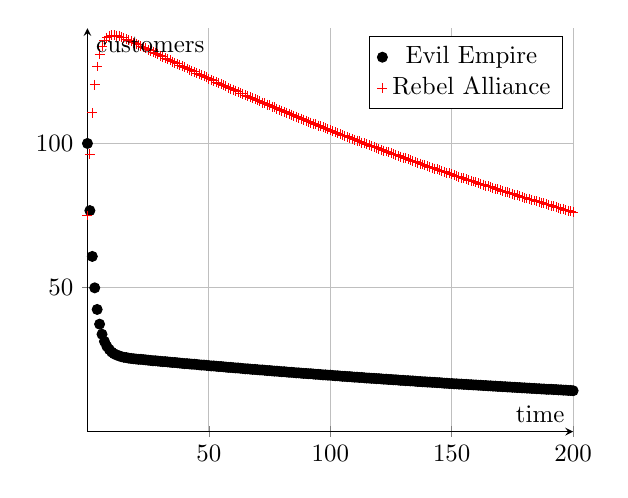
\begin{tikzpicture}[scale=0.9]
            \begin{axis}[grid, axis lines=center, xlabel={time}, ylabel={customers}, ymin=0,
                ymax=140] % , legend pos=outer north east
                \addplot[only marks, mark=*, black] coordinates {(0,100.0)(1  ,76.7) (2  ,60.8) (3  ,49.9) (4  ,42.4) (5  ,37.3) (6  ,33.8) (7  ,31.3) (8  ,29.6) (9  ,28.5) (10 ,27.6) (11 ,27.0) (12 ,26.6) (13 ,26.3) (14 ,26.0) (15 ,25.8) (16 ,25.7) (17 ,25.5) (18 ,25.4) (19 ,25.3) (20 ,25.2) (21 ,25.1) (22 ,25.1) (23 ,25.0) (24 ,24.9) (25 ,24.8) (26 ,24.7) (27 ,24.6) (28 ,24.6) (29 ,24.5) (30 ,24.4) (31 ,24.3) (32 ,24.3) (33 ,24.2) (34 ,24.1) (35 ,24.0) (36 ,24.0) (37 ,23.9) (38 ,23.8) (39 ,23.7) (40 ,23.6) (41 ,23.6) (42 ,23.5) (43 ,23.4) (44 ,23.4) (45 ,23.3) (46 ,23.2) (47 ,23.1) (48 ,23.1) (49 ,23.0) (50 ,22.9) (51 ,22.8) (52 ,22.8) (53 ,22.7) (54 ,22.6) (55 ,22.6) (56 ,22.5) (57 ,22.4) (58 ,22.3) (59 ,22.3) (60 ,22.2) (61 ,22.1) (62 ,22.1) (63 ,22.0) (64 ,21.9) (65 ,21.8) (66 ,21.8) (67 ,21.7) (68 ,21.6) (69 ,21.6) (70 ,21.5) (71 ,21.4) (72 ,21.4) (73 ,21.3) (74 ,21.2) (75 ,21.2) (76 ,21.1) (77 ,21.0) (78 ,21.0) (79 ,20.9) (80 ,20.8) (81 ,20.8) (82 ,20.7) (83 ,20.6) (84 ,20.6) (85 ,20.5) (86 ,20.4) (87 ,20.4) (88 ,20.3) (89 ,20.2) (90 ,20.2) (91 ,20.1) (92 ,20.1) (93 ,20.0) (94 ,19.9) (95 ,19.9) (96 ,19.8) (97 ,19.7) (98 ,19.7) (99 ,19.6) (100,19.6) (101,19.5) (102,19.4) (103,19.4) (104,19.3) (105,19.2) (106,19.2) (107,19.1) (108,19.1) (109,19.0) (110,18.9) (111,18.9) (112,18.8) (113,18.8) (114,18.7) (115,18.6) (116,18.6) (117,18.5) (118,18.5) (119,18.4) (120,18.4) (121,18.3) (122,18.2) (123,18.2) (124,18.1) (125,18.1) (126,18.0) (127,18.0) (128,17.9) (129,17.8) (130,17.8) (131,17.7) (132,17.7) (133,17.6) (134,17.6) (135,17.5) (136,17.4) (137,17.4) (138,17.3) (139,17.3) (140,17.2) (141,17.2) (142,17.1) (143,17.1) (144,17.0) (145,17.0) (146,16.9) (147,16.8) (148,16.8) (149,16.7) (150,16.7) (151,16.6) (152,16.6) (153,16.5) (154,16.5) (155,16.4) (156,16.4) (157,16.3) (158,16.3) (159,16.2) (160,16.2) (161,16.1) (162,16.1) (163,16.0) (164,16.0) (165,15.9) (166,15.9) (167,15.8) (168,15.8) (169,15.7) (170,15.7) (171,15.6) (172,15.6) (173,15.5) (174,15.5) (175,15.4) (176,15.4) (177,15.3) (178,15.3) (179,15.2) (180,15.2) (181,15.1) (182,15.1) (183,15.0) (184,15.0) (185,14.9) (186,14.9) (187,14.8) (188,14.8) (189,14.7) (190,14.7) (191,14.7) (192,14.6) (193,14.6) (194,14.5) (195,14.5) (196,14.4) (197,14.4) (198,14.3) (199,14.3) (200,14.2)};
                \addlegendentry{Evil Empire};
                \addplot[only marks, mark=+, red] coordinates{
(0.00   ,75.00)
(1.00   ,96.25)
(2.00   ,110.6)
(3.00   ,120.3)
(4.00   ,126.7)
(5.00   ,131.0)
(6.00   ,133.8)
(7.00   ,135.6)
(8.00   ,136.6)
(9.00   ,137.2)
(10.00  ,137.5)
(11.00  ,137.5)
(12.00  ,137.4)
(13.00  ,137.2)
(14.00  ,136.9)
(15.00  ,136.6)
(16.00  ,136.2)
(17.00  ,135.8)
(18.00  ,135.4)
(19.00  ,135.0)
(20.00  ,134.6)
(21.00  ,134.2)
(22.00  ,133.8)
(23.00  ,133.4)
(24.00  ,133.0)
(25.00  ,132.5)
(26.00  ,132.1)
(27.00  ,131.7)
(28.00  ,131.3)
(29.00  ,130.9)
(30.00  ,130.5)
(31.00  ,130.1)
(32.00  ,129.6)
(33.00  ,129.2)
(34.00  ,128.8)
(35.00  ,128.4)
(36.00  ,128.0)
(37.00  ,127.6)
(38.00  ,127.2)
(39.00  ,126.8)
(40.00  ,126.4)
(41.00  ,126.0)
(42.00  ,125.6)
(43.00  ,125.2)
(44.00  ,124.8)
(45.00  ,124.4)
(46.00  ,124.0)
(47.00  ,123.6)
(48.00  ,123.3)
(49.00  ,122.9)
(50.00  ,122.5)
(51.00  ,122.1)
(52.00  ,121.7)
(53.00  ,121.3)
(54.00  ,120.9)
(55.00  ,120.6)
(56.00  ,120.2)
(57.00  ,119.8)
(58.00  ,119.4)
(59.00  ,119.0)
(60.00  ,118.7)
(61.00  ,118.3)
(62.00  ,117.9)
(63.00  ,117.5)
(64.00  ,117.2)
(65.00  ,116.8)
(66.00  ,116.4)
(67.00  ,116.1)
(68.00  ,115.7)
(69.00  ,115.3)
(70.00  ,115.0)
(71.00  ,114.6)
(72.00  ,114.2)
(73.00  ,113.9)
(74.00  ,113.5)
(75.00  ,113.2)
(76.00  ,112.8)
(77.00  ,112.5)
(78.00  ,112.1)
(79.00  ,111.7)
(80.00  ,111.4)
(81.00  ,111.0)
(82.00  ,110.7)
(83.00  ,110.3)
(84.00  ,110.0)
(85.00  ,109.6)
(86.00  ,109.3)
(87.00  ,108.9)
(88.00  ,108.6)
(89.00  ,108.3)
(90.00  ,107.9)
(91.00  ,107.6)
(92.00  ,107.2)
(93.00  ,106.9)
(94.00  ,106.6)
(95.00  ,106.2)
(96.00  ,105.9)
(97.00  ,105.6)
(98.00  ,105.2)
(99.00  ,104.9)
(100.00 ,104.6)
(101.00 ,104.2)
(102.00 ,103.9)
(103.00 ,103.6)
(104.00 ,103.2)
(105.00 ,102.9)
(106.00 ,102.6)
(107.00 ,102.3)
(108.00 ,101.9)
(109.00 ,101.6)
(110.00 ,101.3)
(111.00 ,101.0)
(112.00 ,100.7)
(113.00 ,100.3)
(114.00 ,100.0)
(115.00 ,99.7)
(116.00 ,99.4)
(117.00 ,99.1)
(118.00 ,98.8)
(119.00 ,98.5)
(120.00 ,98.2)
(121.00 ,97.8)
(122.00 ,97.5)
(123.00 ,97.2)
(124.00 ,96.9)
(125.00 ,96.6)
(126.00 ,96.3)
(127.00 ,96.0)
(128.00 ,95.7)
(129.00 ,95.4)
(130.00 ,95.1)
(131.00 ,94.8)
(132.00 ,94.5)
(133.00 ,94.2)
(134.00 ,93.9)
(135.00 ,93.6)
(136.00 ,93.3)
(137.00 ,93.0)
(138.00 ,92.7)
(139.00 ,92.4)
(140.00 ,92.1)
(141.00 ,91.8)
(142.00 ,91.6)
(143.00 ,91.3)
(144.00 ,91.0)
(145.00 ,90.7)
(146.00 ,90.4)
(147.00 ,90.1)
(148.00 ,89.8)
(149.00 ,89.6)
(150.00 ,89.3)
(151.00 ,89.0)
(152.00 ,88.7)
(153.00 ,88.4)
(154.00 ,88.1)
(155.00 ,87.9)
(156.00 ,87.6)
(157.00 ,87.3)
(158.00 ,87.0)
(159.00 ,86.8)
(160.00 ,86.5)
(161.00 ,86.2)
(162.00 ,85.9)
(163.00 ,85.7)
(164.00 ,85.4)
(165.00 ,85.1)
(166.00 ,84.9)
(167.00 ,84.6)
(168.00 ,84.3)
(169.00 ,84.1)
(170.00 ,83.8)
(171.00 ,83.5)
(172.00 ,83.3)
(173.00 ,83.0)
(174.00 ,82.7)
(175.00 ,82.5)
(176.00 ,82.2)
(177.00 ,82.0)
(178.00 ,81.7)
(179.00 ,81.4)
(180.00 ,81.2)
(181.00 ,80.9)
(182.00 ,80.7)
(183.00 ,80.4)
(184.00 ,80.2)
(185.00 ,79.9)
(186.00 ,79.7)
(187.00 ,79.4)
(188.00 ,79.2)
(189.00 ,78.9)
(190.00 ,78.7)
(191.00 ,78.4)
(192.00 ,78.2)
(193.00 ,77.9)
(194.00 ,77.7)
(195.00 ,77.4)
(196.00 ,77.2)
(197.00 ,76.9)
(198.00 ,76.7)
(199.00 ,76.5)
(200.00 ,76.2)};
                \addlegendentry{Rebel Alliance};
            \end{axis}
        \end{tikzpicture}
        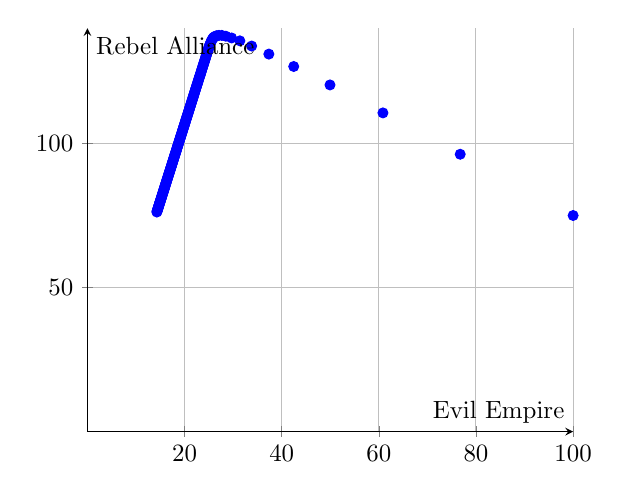
\begin{tikzpicture}[scale=0.9]
            \begin{axis}[grid, axis lines=center, xlabel={Evil Empire}, ylabel={Rebel Alliance},
                ymin=0, ymax=140, xmin=0]
                \addplot[blue, only marks, mark=*] coordinates {
(100.00 ,75.00)
(76.75  ,96.25)
(60.84  ,110.6)
(49.94  ,120.3)
(42.47  ,126.7)
(37.35  ,131.0)
(33.81  ,133.8)
(31.38  ,135.6)
(29.68  ,136.6)
(28.50  ,137.2)
(27.67  ,137.5)
(27.07  ,137.5)
(26.64  ,137.4)
(26.32  ,137.2)
(26.08  ,136.9)
(25.88  ,136.6)
(25.73  ,136.2)
(25.59  ,135.8)
(25.48  ,135.4)
(25.37  ,135.0)
(25.28  ,134.6)
(25.19  ,134.2)
(25.10  ,133.8)
(25.01  ,133.4)
(24.93  ,133.0)
(24.85  ,132.5)
(24.77  ,132.1)
(24.69  ,131.7)
(24.61  ,131.3)
(24.53  ,130.9)
(24.46  ,130.5)
(24.38  ,130.1)
(24.30  ,129.6)
(24.22  ,129.2)
(24.15  ,128.8)
(24.07  ,128.4)
(24.00  ,128.0)
(23.92  ,127.6)
(23.84  ,127.2)
(23.77  ,126.8)
(23.69  ,126.4)
(23.62  ,126.0)
(23.54  ,125.6)
(23.47  ,125.2)
(23.40  ,124.8)
(23.32  ,124.4)
(23.25  ,124.0)
(23.18  ,123.6)
(23.10  ,123.3)
(23.03  ,122.9)
(22.96  ,122.5)
(22.88  ,122.1)
(22.81  ,121.7)
(22.74  ,121.3)
(22.67  ,120.9)
(22.60  ,120.6)
(22.53  ,120.2)
(22.45  ,119.8)
(22.38  ,119.4)
(22.31  ,119.0)
(22.24  ,118.7)
(22.17  ,118.3)
(22.10  ,117.9)
(22.03  ,117.5)
(21.96  ,117.2)
(21.89  ,116.8)
(21.82  ,116.4)
(21.76  ,116.1)
(21.69  ,115.7)
(21.62  ,115.3)
(21.55  ,115.0)
(21.48  ,114.6)
(21.41  ,114.2)
(21.35  ,113.9)
(21.28  ,113.5)
(21.21  ,113.2)
(21.15  ,112.8)
(21.08  ,112.5)
(21.01  ,112.1)
(20.95  ,111.7)
(20.88  ,111.4)
(20.81  ,111.0)
(20.75  ,110.7)
(20.68  ,110.3)
(20.62  ,110.0)
(20.55  ,109.6)
(20.49  ,109.3)
(20.42  ,108.9)
(20.36  ,108.6)
(20.29  ,108.3)
(20.23  ,107.9)
(20.17  ,107.6)
(20.10  ,107.2)
(20.04  ,106.9)
(19.98  ,106.6)
(19.91  ,106.2)
(19.85  ,105.9)
(19.79  ,105.6)
(19.72  ,105.2)
(19.66  ,104.9)
(19.60  ,104.6)
(19.54  ,104.2)
(19.48  ,103.9)
(19.42  ,103.6)
(19.35  ,103.2)
(19.29  ,102.9)
(19.23  ,102.6)
(19.17  ,102.3)
(19.11  ,101.9)
(19.05  ,101.6)
(18.99  ,101.3)
(18.93  ,101.0)
(18.87  ,100.7)
(18.81  ,100.3)
(18.75  ,100.0)
(18.69  ,99.7)
(18.63  ,99.4)
(18.58  ,99.1)
(18.52  ,98.8)
(18.46  ,98.5)
(18.40  ,98.2)
(18.34  ,97.8)
(18.28  ,97.5)
(18.23  ,97.2)
(18.17  ,96.9)
(18.11  ,96.6)
(18.05  ,96.3)
(18.00  ,96.0)
(17.94  ,95.7)
(17.88  ,95.4)
(17.83  ,95.1)
(17.77  ,94.8)
(17.71  ,94.5)
(17.66  ,94.2)
(17.60  ,93.9)
(17.55  ,93.6)
(17.49  ,93.3)
(17.44  ,93.0)
(17.38  ,92.7)
(17.33  ,92.4)
(17.27  ,92.1)
(17.22  ,91.8)
(17.16  ,91.6)
(17.11  ,91.3)
(17.06  ,91.0)
(17.00  ,90.7)
(16.95  ,90.4)
(16.89  ,90.1)
(16.84  ,89.8)
(16.79  ,89.6)
(16.74  ,89.3)
(16.68  ,89.0)
(16.63  ,88.7)
(16.58  ,88.4)
(16.52  ,88.1)
(16.47  ,87.9)
(16.42  ,87.6)
(16.37  ,87.3)
(16.32  ,87.0)
(16.27  ,86.8)
(16.21  ,86.5)
(16.16  ,86.2)
(16.11  ,85.9)
(16.06  ,85.7)
(16.01  ,85.4)
(15.96  ,85.1)
(15.91  ,84.9)
(15.86  ,84.6)
(15.81  ,84.3)
(15.76  ,84.1)
(15.71  ,83.8)
(15.66  ,83.5)
(15.61  ,83.3)
(15.56  ,83.0)
(15.51  ,82.7)
(15.46  ,82.5)
(15.41  ,82.2)
(15.37  ,82.0)
(15.32  ,81.7)
(15.27  ,81.4)
(15.22  ,81.2)
(15.17  ,80.9)
(15.13  ,80.7)
(15.08  ,80.4)
(15.03  ,80.2)
(14.98  ,79.9)
(14.93  ,79.7)
(14.89  ,79.4)
(14.84  ,79.2)
(14.79  ,78.9)
(14.75  ,78.7)
(14.70  ,78.4)
(14.65  ,78.2)
(14.61  ,77.9)
(14.56  ,77.7)
(14.52  ,77.4)
(14.47  ,77.2)
(14.42  ,76.9)
(14.38  ,76.7)
(14.33  ,76.5)
(14.29  ,76.2) };
            \end{axis}
        \end{tikzpicture}
    \end{center}
    \caption{Evil empire customers and Rebel Alliance customers over a 200 week time
    period.}
    \label{fig:10.8.empire1}
\end{figure}

% \input{activities/10.8.Act1}
\begin{problem}
    Find the general solution to the two problems from Section \ref{sec:linear_systems}.
\end{problem}



\subsection{Analysis of Equilibrium Behavior}
The equilibrium solution of a difference equation occurs when the new term $\bx_{k+1}$ is
equal to the old term $\bx_k$.  If the system of difference equations is $\bx_{k+1} = A
\bx_{k}$ then to find the equilibrium solution we need to solve $\bx_{e} = A \bx_e$.  The
reader should recognize this as either the hunt for the eigenvalue $\lambda=1$ and its
associated eigenvector, or the zero vector.  Remember that not every matrix will have a
unit eigenvalue and we don't call the zero vector an eigenvector.  Even so, the zero
vector will be an equilibrium point since it is the trivial solution to $\bx_e = A \bx_e$.

% For the $2 \times 2$ matrix $A = \bpm a & b \\ c & d \epm$ we can do some of the work
% symbolically to try and extract all of the necessary information.  First, $\det(A-\lambda
% I)$ is
% \[ \det(A-\lambda I) = \det\left( \bpm a-\lambda & b \\ c & d-\lambda \epm \right) =
% (a-\lambda)(d-\lambda) - bc = ad - a\lambda - d\lambda + \lambda^2 - bc. \]
% After a bit of rearranging, the characteristic polynomial is
% \[ p(\lambda) = \det(A - \lambda I) = \lambda^2 - (a+d)\lambda + \left( ad-bc \right). \]
% \begin{definition}
%     Consider a $2 \times 2$ matrix $A = \bpm a & b \\ c & d \epm$.
%     \begin{itemize}
%         \item The {\bf trace} of a matrix is the sum of the diagonal entries:
%             \[ \text{trace}(A) = \text{tr}\bpm a & b \\ c & d \epm = a+d. \]
% 
%         \item The {\bf characteristic polynomial} of $A$ is
%             \[ p(\lambda) = \lambda^2 - \text{tr}(A) \lambda + \det(A).\]
%         
%         \item The eigenvalues of $A$ are
%             \[ \lambda_{1,2} = \frac{\text{tr}(A) \pm
%             \sqrt{[\text{tr}(A)]^2-4\det(A)}}{2}. \]
%     \end{itemize}
% 
%     \label{def:10.8.char_poly}
% \end{definition}

\begin{thm}
    To determine the stability of the origin in the discrete dynamical system
    $\bx_{k+1}=A\bx_k$ we have several cases related to the two eigenvalues $\lambda_1$
    and $\lambda_2$:

    \begin{enumerate}
        \item If $|\lambda_1|<1$ and $|\lambda_2|<1$ then the origin is stable.
        \item If either $|\lambda_1|>1$ or $|\lambda_2|>1$ then the origin is unstable.
        \item If $\lambda_1=1$ and 
            \begin{itemize}
                \item $\lambda_2=1$ then there is no equilibrium solution
                \item $|\lambda_2|<1$ then the origin is unstable and the equilibrium is a
                    multiple of the eigenvector associated with $\lambda_1=1$.
                \item $\lambda_2=-1$ then there may or may not be an equilibrium.  If
                    there is an equilibrium then it is unstable.
            \end{itemize}

    \end{enumerate}
\end{thm}

% Using the definition of the characteristic polynomial \ref{def:10.8.char_poly} a thorough
% description of the dynamics of the system can be extracted by the discriminant of the
% quadratic formula: $[\text{tr}(A)]^2-4\det(A)$.  In Figure \ref{fig:10.8.trace_det}, the
% parabola is a plot of $[\text{tr}(A)]^2-4\det(A)=0$, and this curve naturally divides the
% trace-determinant space into several regions (indicated by the color markers).  
% 
% \begin{figure}[ht!]
%     \centering
%     \begin{tikzpicture}
%         \begin{axis}[axis lines=center, xlabel={$\text{tr}(A)$}, ylabel={$\det(A)$}, 
%             xmax=4, xmin=-4, ymin=-1, ymax=3, legend pos=outer north east, xtick=\empty,
%         ytick=\empty]
%             \addplot[smooth, very thick, black, domain=-4:4] {x^2/4};
%             \addlegendentry{$(\text{tr}(A))^2-4\det(A)=0$};
%             %
%             \addplot[only marks, mark=o, red] coordinates{(-3,1)};
%             \addlegendentry{$\text{tr}(A)<0$ and $4\det(A)<[\text{tr}(A)]^2$};
%             %
%             \addplot[only marks, mark=otimes, cyan] coordinates{(-1,2)};
%             \addlegendentry{$\text{tr}(A)<0$ and $4\det(A)>[\text{tr}(A)]^2$};
%             %
%             \addplot[only marks, mark=star, black] coordinates{(0,1.5)};
%             \addlegendentry{$\text{tr}(A)=0$ and $\det(A)>0$};
%             %
%             \addplot[only marks, mark=+, magenta] coordinates{(1,2)};
%             \addlegendentry{$\text{tr}(A)>0$ and $4\det(A)>[\text{tr}(A)]^2$};
%             %
%             \addplot[only marks, mark=*, blue] coordinates{(3,1)};
%             \addlegendentry{$\text{tr}(A)>0$ and $4\det(A)<[\text{tr}(A)]^2$};
%             %
%             \addplot[only marks, mark=oplus, green!50!black] coordinates{(1,-0.5)};
%             \addlegendentry{$\text{tr}(A)>0$ and $\det(A)<0$};
%             %
%             \addplot[only marks, mark=diamond, cyan!30!black] coordinates{(-1,-0.5)};
%             \addlegendentry{$\text{tr}(A)<0$ and $\det(A)<0$};
%             %
%             \addplot[only marks, mark=*, red!70!blue] coordinates{(1,0.25)};
%             \addlegendentry{$\text{tr}(A)>0$ and $4\det(A)=[\text{tr}(A)]^2$};
%             %
%             \addplot[only marks, mark=o, blue!30!red] coordinates{(-1,0.25)};
%             \addlegendentry{$\text{tr}(A)<0$ and $4\det(A)=[\text{tr}(A)]^2$};
%             %
%             \addplot[only marks, mark=square, green!30!red] coordinates{(1.5,0)};
%             \addlegendentry{$\text{tr}(A)>0$ and $\det(A)=0$};
%             %
%             \addplot[only marks, mark=square, color=red!30!green] coordinates{(-1.5,0)};
%             \addlegendentry{$\text{tr}(A)<0$ and $\det(A)=0$};
%             %
%         \end{axis}
%     \end{tikzpicture}
%     \caption{Schematic of the different possible eigenvalue behavior in a $2 \times 2$
%     discrete dynamical system. Each mark represents a region where the behavior of the
% system is potentially different from other regions.}
%     \label{fig:10.8.trace_det}
% \end{figure}
%




% 
% \input{activities/10.8.Act2}
% \begin{problem}
%     Let $A = \bpm a & b \\ c & d \epm$ and consider the discrete dynamical system
%     $\bx_{k+1} = A \bx_k$.
% 
%     {\bf Your Task:} 
%     \begin{itemize}
%         \item Use the GeoGebra applet
%             \href{http://www.geogebratube.org/student/m306119}{http://www.geogebratube.org/student/m306119}
%             to experiment with various $2\times 2$ discrete dynamical systems.
%         \item Determine the behavior of each of the regions in Figure
%             \ref{fig:10.8.trace_det}. In each case, describe the equilibrium point(s) and
%             their stability.
%         \item Hint: The simplest place to start is with a matrix of the form $A = \bpm
%             \lambda_1 & 0 \\ 0 & \lambda_2 \epm$.  You won't be able to use this form for
%             every region of Figure \ref{fig:10.8.trace_det}, but it will get you started.
%     \end{itemize}
% \end{problem}
% 


\begin{example}
Consider the system of difference equations 
\begin{flalign*}
    a_{n+1} &= 2a_n - b_n \\
    b_{n+1} &= -4a_n - b_n \\
    a_0 &= 1 \\
    b_0 &= -6
\end{flalign*}
Write the system as a matrix equation and write the solution as a linear combination of
the eigenvectors.
\\{\bf Solution:}\\
The matrix form of the equation is 
\[ \underbrace{\bpm a_{n+1} \\ b_{n+1} \epm}_{\bx_{n+1}} = \underbrace{\bpm 2 & -1 \\ -4 &
-1 \epm}_{A} \underbrace{\bpm a_n \\ b_n \epm}_{\bx_n} \quad \text{with} \quad \bx_0 =
\bpm 1 \\ -6 \epm \]

Recall that the analytic solution to this difference equation is
\[ \bx_n = A^n \bx_0. \]
In order to efficiently evaluate the matrix power we find the eigenvalue-eigenvector
pairs.  After some work, the eigenvalues and eigenvectors of the coefficient matrix $A$
are $\lambda_1 = 3$ with $\bv_1 = \bpm 1 \\ -1 \epm$ and $\lambda_2 = -2$ with $\bv_2 =
\bpm 1 \\ 4 \epm$.  Therefore
\[ \bx_n = C_1 \cdot 3^n \cdot \bpm 1 \\ -1 \epm + C_2 \cdot (-2)^n \cdot \bpm 1 \\ 4
\epm. \]
Given that $\lambda_1=3$ and $\lambda_2=-2$ we know that the equilibrium solution
$\bx=0$ will be unstable.

It only remains to find the constants.  The constants come from observing that $\bx_0 =
C_1 \bv_1 + C_2 \bv_2$.  This is a system of equations, and in augmented form we see that 
\[ \left( \begin{array}{cc|c} 1 & 1 & 1 \\ -1 & 4 & -6 \end{array} \right) \to \left(
    \begin{array}{cc|c} 1 & 0 & 2 \\ 0 & 1 & -1 \end{array} \right) \implies \left\{
    \begin{array}{l} c_1=2 \\ c_2=-1 \end{array} \right. \]
Therefore, the final solution to the discrete dynamical system is
\[ \bx_n = \bpm a_n \\ b_n \epm =  2 \cdot 3^n \bpm 1 \\ -1 \epm + (-1) \cdot (-2)^n \bpm
1 \\ 4 \epm = \bpm 2\cdot 3^n - (-2)^n \\ -2 \cdot 3^n - 4\cdot (-2)^n \epm. \]
This solution can easily be plotted with a graphing utility (we leave this to the reader).
\end{example}


% \input{activities/10.8.Act3}
\begin{problem}
    For each of the problems below, find the general solution to the difference equation
    and discuss the stability of the origin.

    \ba
        \item $A = \bpm 1/2 & 1/4 \\ 1/4 & 1/2 \epm$ with $\bx_0 = \bpm 1\\1 \epm$.  The
            eigen-pairs for $A$ are
            \[ \lambda_1=0.75 \text{ with } \bv_1 = \bpm 1 \\ 1 \epm \quad \text{and}
            \quad \lambda_2 = 0.25 \text{ with } \bv_2 = \bpm -1 \\ 1 \epm. \]
        \item $A = \bpm 2 & -1 \\ 0 & 3 \epm$ with $\bx_0 = \bpm 4 \\ 1 \epm$.  The
            eigen-pairs are
            \[ \lambda_1 = 3 \text{ with } \bv_1 = \bpm -1 \\ 1 \epm \quad \text{ and
            }\quad \lambda_2 = 2 \text{ with } \bv_2 = \bpm 1 \\ 0 \epm. \]
        \item $A = \bpm 7 & 0 & 5 \\ 0 & 5 & 0 \\ -4 & 0 & -2 \epm$ with $\bx_0 = \bpm 9
            \\ -2 \\ -8 \epm$.  Hint: The eigen-pairs are
            \[ \lambda_1=3 \text{ with } \bv_1 = \bpm 5 \\ 0 \\ -4 \epm, \quad \lambda_2 =
                2 \text{ with } \bv_2 = \bpm -1 \\ 0 \\ 1 \epm, \quad \text{and} \quad
            \lambda_3 = 5 \text{ with } \bv_3 = \bpm 0 \\ 5 \\ 0 \epm. \]
    \ea
    
\end{problem}




\subsection{Non Homogeneous Systems of Linear Difference Equations}
Now that we have an intuitive sense of how complicated the dynamics of a linear
homogeneous system can be, let's dive into the least complicated non-homogeneous dynamical
system:
\[ \bx_{k+1} = A \bx_k + \bb \]

An equilibrium solution to occurs when $\bx_{k+1} = \bx_k$.  In other words, we need to
solve
\[ \bx_e = A \bx_e + \bb. \]
Unlike the homogeneous system, in this case we can use (linear) algebra to rearrange:
\[ \bx_e = A \bx_e + \bb \quad \implies \quad \bx_e - A \bx_e = \bb \quad \implies
\quad (I-A)\bx_e = \bb. \]
On paper, the equilibrium vector is $\bx_e = (I-A)^{-1} \bb$.  As discussed previously,
inverting a matrix is often not a great ideal so it may be necessary to lean on some
linear algebra technology to solve the system for $\bx_e$.  The eigenvalue structure of
$A$ tells you complete information about the stability of the equilibrium point as it did
in the homogeneous case.  In general, if $\bb$ is not constant then the system will
likely not have an equilibrium point.

\begin{thm}
    Let $\bx_{n+1} = A \bx_n + \bb$ be a non-homogeneous system of linear difference
    equations.  If $A$ has eigen-pairs $\lambda_1, \bv_1$, $\lambda_2, \bv_2$, \dots,
    $\lambda_k, \bv_k$ and the initial condition $\bx_0$ can be written as $\bx_0 = C_1
    \bv_1 + C_2 \bv_2 + \cdots + C_k \bv_k + \bx_e$ then the general solution to the
    non-homogeneous system of difference equations is
    \[ \bx_n = \left( C_1 \lambda_1^n \bv_1 + C_2 \lambda_2^n \bv_n + \cdots C_k
    \lambda_k^n \bv_k \right) + \bx_e \]
    where $\bx_e$ is the equilibrium solution $\bx_e = (I-A)^{-1} \bb$.
    \label{thm:10.8.gen_soln_nonhom}
\end{thm}

\begin{example}
Consider the system of equation 
\[ \bx_{n+1} = \bpm a_{n+1} \\ b_{n+1} \epm = \bpm 1 & 0.75 \\ -0.5 & -0.25 \epm \bpm a_n
\\ b_n \epm + \bpm 1 \\ 0 \epm. \]
Find the general solution to the system of equation with the initial condition $\bx_0 =
\bpm 1 \\ 2 \epm$.
\\{\bf Solution:}\\
The eigen-pairs for the matrix $A$ are
\[ \lambda_1 = 0.25 \text{ with } \bv_1 = \bpm -1\\1\epm \quad \text{and} \quad \lambda_2
= 0.5 \text{ with } \bv_2 = \bpm 3 \\ -2 \epm. \]
Furthermore, the equilibrium point is $\bx_e = (I-A)^{-1} \bb$ where $\bb = \bpm 1
\\ 0 \epm$.  Hence,
\[ \bx_e = \bpm 10/3 \\ -4/3 \epm. \]

Therefore, the general solution to the system of difference equations is
\[ \bx_n = C_1 (0.25)^n \bpm -1 \\ 1 \epm + C_2 (0.5)^n \bpm 3 \\ -2 \epm + \bpm 10/3 \\
-4/3 \epm. \]
Since both eigenvalues are less than 1 and greater than zero the long term behavior of the
system will tend toward the equilibrium, so
\[ \lim_{n \to \infty} \bx_n = \bpm 10/3 \\ -4/3 \epm. \]
In other words, $\bx_e$ is a stable equilibrium.

To solve the system of equation with the given initial condition we observe the system of
equations $\bx_0 = C_1 \bv_1 + C_2 \bv_2 + \bpm 10/3 \\ -4/3 \epm$, augment, and row
reduce to find $C_1=16/3$ and
$C_2=1$.  Therefore,
\[ \bx_n = \left( \frac{16}{3} \right) (0.25)^n \bpm -1 \\ 1 \epm + 1 (0.5)^n \bpm 3 \\ -2 \epm + \bpm 10/3 \\
-4/3 \epm. \]
\end{example}

% \input{activities/10.8.Act4}
\begin{problem}
    For each of the problems below, find the general solution to the difference equation
    and discuss the stability of any equilibrium points.  Use linear algebra software
    where appropriate.

    \ba
\item Consider the system of difference equations
    \begin{flalign*}
        \bpm a_{n+1} \\ b_{n+1} \epm &= \bpm 0.2 & 0.6 \\ 0.3 & 0.1 \epm \bpm a_n \\ b_n
        \epm + \bpm -18 \\ 27
        \epm \quad \text{ with } \quad \bpm a_0 \\ b_0 \epm = \bpm 0 \\ 28 \epm
    \end{flalign*}

\item Consider the system of difference equations
    \begin{flalign*}
        \bpm a_{n+1} \\ b_{n+1} \\ c_{n+1} \epm &= \bpm 0.1 & 0.1 & 0.3 \\ 0.1 & 0.3 & 0.1
        \\ 0.3  & 0.1 & 0.1 \epm \bpm a_n \\ b_n \\ c_n \epm + \bpm -96 \\ -24 \\ -120
        \epm \quad \text{ with } \quad \bpm a_0 \\ b_0 \\ c_0 \epm = \bpm -226 \\ -45 \\
        -218 \epm
    \end{flalign*}
    \ea
    
\end{problem}





\newpage\section{Modeling Explorations with Systems}
\begin{problem}[Deer and Cougar Problem]
We are going to build a difference equation model that predicts the populations of cougars
$C$ and deer $D$ (predators and prey) at year $t$
\begin{enumerate}
    \item {\bf The Mathematical Model:} 
        \begin{enumerate}
            \item {\bf Deer Population:} The change in deer population can be modeled as 
                \[ D'(t) = (\text{logistic population growth}) - (\text{deer removed
                by interactions with cougars}) \]
                \begin{itemize}
                    \item a generic logistic growth difference equation takes the form: 
                        \[ y'(t) = k y \left(1-\frac{y}{N}\right) \]
                        where $k$ is the growth rate parameter and
                        $N$ is the carrying capacity of the population.
                    \item Assume that the carrying capacity for the deer is $N = 4,500$,
                        and assume that $k \approx 0.3$
                    \item The rate at which the deer population is removed due to
                        interactions with cougars is proportional to the product of the
                        deer and cougar populations.  Assume that the proporationality
                        constant is $-0.15$.
                    \item Write the differential equation for the deer population. 
                \end{itemize}
            \item {\bf Cougar Population:} The change in cougar population can be modeled
                as
                \[ C'(t) = \left( \text{natural death rate} \right) + \left(
                    \text{gain due to abundance of food source}
                \right) \]
                \begin{itemize}
                    \item Assume that the natural death rate for the cougar population is
                        proportional to the current number of cougars.  Let the
                        proportionality constant be $-0.30$.
                    \item Assume that the gain in population is proportional to the
                        product of the deer and cougar populations with proportionality
                        constant $0.00015$.
                    \item Write the difference equation for the cougar population.
                \end{itemize}
            \item {\bf The Model:} The two difference equations that you've written along
                with the initial conditions $D_0 = 500$ and $C_0 = 2$ are now your
                mathematical model!  Summarize them in one place in your lab.
        \end{enumerate}
    \item {\bf Model Description:} Describe some features of this model by answering the following questions.
        (please restate the questions in your lab writeup)
        \begin{enumerate}
            \item Which animal is the predator and which is the prey? 
            \item What is the significance of the $+$ sign in the equation for cougars? 
            \item What is the significance of the $-$ sign in the equation for deer? 
            \item In the absence of deer, does the cougar population increase or decrease?
                At what rate?
            \item In the absence of cougars, does the deer population increase or
                decrease? At what rate?
            \item How many deer does each cougar consume when there are 1000 deer vs when
                there are 2000 deer?
        \end{enumerate}

    \item {\bf Numerical Solution:}  Construct a numerical solution to this system of
        difference equations.  Recall that a numerical solution for a differential
        equation model will use Euler's method.  This time you'll need to build both
        equations simultaneously.  Your numerical approximation will give you both the
        deer population and the cougar population.
        For a system of differential equations there are three appropriate plots that you
        need to generate.
        \begin{description}
            \item[Deer vs Time:] Plot the number of deer on the $y$ axis and time ($t$) on the
                $x$ axis.
            \item[Cougars vs Time:] Plot the number of cougars on the $y$ axis and time ($t$) on the
                $x$ axis.
            \item[Deer vs Cougars:] Plot the number of deer on the $y$ axis and the number
                of cougars on the $x$ axis (or visa versa).  This is called the phase
                plot.
        \end{description}
        Write a paragraph describing the behavior of the deer and cougar populations over
        the course of 100 years. Identify each of the key features\footnote{{\it Key
        features} would include maximums, minimums, regions of increase or decrease,
    extinction, overpopulation, equilibrium, etc.} of the population dynamics.

    \item {\bf Analysis:} 
        \begin{enumerate}
            \item There are several assumptions in this model, but in particular we have
                assumed that the cougar population will only go up via direct interactions
                with prey (deer).  Change the death rate term in the cougar population to
                a plausible model that depends on the current number of cougars.  Repeat
                the numerical solutions for several possible parameters.
            \item Is either model (the original or the new from part (a)) sensitive to
                initial conditions?  Vary each initial condition slightly and discuss how
                the dynamical system behaves. Support your disucssion with appropriate
                plots or tables.
            \item There are {\it interaction terms} in each equation of the model (the
                terms involving both $C$ and $D$).  How sensitive is the model to the
                interaction rate $0.15$?  Vary this interaction term slightly and discuss
                the behavior of the dynamical system. Support your discussion with
                appropriate plots or tables.
            \item Attack several other assumptions built into this model, make the
                appropriate changes to the model, and determine what the impact is on the
                resulting populations.
        \end{enumerate}



    \item Write an Executive Summary describing what you did in this lab.  This is meant
        to be a reference to you when you need to re-use the ideas (both mathematical and
        computational) from this lab. Your executive summary should be immediately under
        the title on the front page of the lab.  It should be no more than a paragraph or
        two, and it should make for easy reference later.

\end{enumerate}
\end{problem}

\begin{problem}[The Bedridden Boys Problem]
A boarding school is a relatively closed community in which all students live on campus,
teachers tend to live on or near campus, and students do not regularly interact with
people not in the boarding school community. The data set in Table
\ref{tab:bedridden_boys} gives data for an influenza
outbreak at a boarding school in England during which there were no fatalities. There were
763 boys at the English boarding school from which the data was obtained. This is only one
instance of the types of influenza outbreaks that occur every year at boarding schools and
on college campuses.  {\bf Create a mathematical model for the number of infected people
    in a closed community (such as a dorm or boarding school) as a function of time.}
    Assume there is 1 person initially infected.

What makes this situation interesting:
\begin{itemize}
    \item People don't generally show symptoms right away after they are exposed to a virus.
    \item Some people may have been previously exposed to the virus and are therefore
        immune.
    \item In a closed community it may or may not be possible to implement a quarantine.
    \item Some people will not admit themselves for medical care even though they are
        infected.  Hence, those people will likely not be counted in medical records for
        the outbreak.
    \item \ldots and many others \ldots
\end{itemize}
Your Tasks:
\begin{itemize}
    \item[(a)]create, solve, and analyze a simple model (with as many assumptions as
        necessary),
    \item[(b)] refine your model to either reduce the number of assumptions or to increase the
        complexity (and hence make the model more realistic), and
    \item[(c)] refine the model a second time to create an even more realistic model.
\end{itemize}
At each step your group must do a thorough analysis of the mathematical model.  This
includes a sensitivity analysis for any model parameters. The modeling process will
require your group to research the real problem to determine the assumptions and any
necessary terminology. Be sure to properly cite any sources used and to check the
reliability of those sources.
\end{problem}

\begin{table}[ht!]
    \centering
    \begin{tabular}{|c|c|}
        \hline
       Time (in days) &  Number of Bedridden Boys \\ \hline \hline
       0  & 1\\\hline
       1  & 3\\\hline
       2  & 25\\\hline
       3  & 72\\\hline
       4  & 222\\\hline
       5  & 282\\\hline
       6  & 256\\\hline
       7  & 233\\\hline
       8  & 189\\\hline
       9  & 123\\\hline
       10 & 70\\\hline
       11 & 25\\\hline
       12 & 11\\\hline
       13 & 4\\\hline
    \end{tabular}
    \caption{Bedridden Boys Data}
    \label{tab:bedridden_boys}
\end{table}


\begin{problem}[The Ibuprofen Problem]
Ibuprofen, an analgesic pain reliever, is ingested into the gastrointestinal tract by
swallowing a pill of the substance or drinking a solution.  The drug then moves to the
plasma or serum where it travels to sites to do its work of pain relief.  {\bf Create a
    mathematical model for the concentration of the Ibuprofen (in $\mu$g/ml) in the plasma
as a function of time.} The data set in Table \ref{tab:ibuprofen_data} gives one patient's Ibuprofen concentration over time
with a 400 mg initial dose.

What makes this situation interesting:
\begin{itemize}
    \item The Ibuprofen doesn't actually move directly into the plasma.
    \item The units of the dose are milligrams (typically, 400mg) but the units of the
        concentration are micro grams per milliliter.
    \item The volume of the gastrointestinal tract and the plasma are different.
    \item Every person's body will metabolize Ibuprofen at different rates.
    \item As the effects of the drug wear off the patient usually takes more Ibuprofen.
    \item \ldots and many others \ldots
\end{itemize}
Your Tasks:
\begin{itemize}
    \item[(a)]create, solve, and analyze a simple model (with as many assumptions as
        necessary),
    \item[(b)] refine your model to either reduce the number of assumptions or to increase the
        complexity (and hence make the model more realistic), and
    \item[(c)] refine the model a second time to create an even more realistic model.
\end{itemize}
At each step your group must do a thorough analysis of the mathematical model.  This
includes a sensitivity analysis for any model parameters. The modeling process will
require your group to research the real problem to determine the assumptions and any
necessary terminology. Be sure to properly cite any sources used and to check the
reliability of those sources.
\end{problem}


\begin{table}[ht!]
    \centering
    \begin{tabular}{|c|c|}
        \hline
Time (hours)  &  Ibuprofen Concentration in Plasma (micro grams / ml) \\ \hline \hline
0  & 0 \\\hline
0.0833 &  12.5 \\\hline
0.167  & 26.5 \\\hline
0.25  & 33 \\\hline
0.33 &  37.4 \\\hline
0.5 &  36.2 \\\hline
1  & 33.2 \\\hline
1.5 &  30.2 \\\hline
2  & 23.9 \\\hline
3  & 16.3 \\\hline
4  & 11.7 \\\hline
6  & 5.82 \\\hline
8  & 3.09 \\\hline
    \end{tabular}
    \caption{Ibuprofen Data}
    \label{tab:ibuprofen_data}
\end{table}
